%% Diese Vorlage wurde am 24.08.2021 von Teresa Seidl Fernández erstellt 
%% und wird den Studenten/-innen der Fakultät für Angewandte Psychologie
%% der SRH Hochschule zur Verfügung gestellt und kann auch von ihnen
%% angepasst werden.






%%%%%%%%%%%%%%%%%%%%%%%%%%%% VORSPANN %%%%%%%%%%%%%%%%%%%%%%%%%

\documentclass[12pt, a4paper]{report}

\usepackage{SRH_Vorlage}

\usepackage[ngerman]{babel}        % n steht für neu und richtet sich an den
% neuen Rechtschreibregeln. Weitere Sprachen können verwendet werden. Um eine
% dieser Sprachen als "Hauptsprache" zu determinieren: main=[gewünschte Sprache]
\usepackage{ifthen}     % The package’s basic command is \ifthenelse, which 
% can use a wide array of tests. Also provided is a simple loop command 
% \whiledo. Ifthen is a separate package within the LaTeX distribution; 
% while it will always be present in a LaTeX distribution, a \usepackage 
% command is always needed to load it. 
\usepackage[retainmissing]{MnSymbol}    % MnSymbol is a symbol font family.
%  Almost all of LaTeX and AMS mathematical symbols are provided
\usepackage{titletoc}     % Alternative headings for toc/lof/lot
% Anhang:
\usepackage[titletoc,title]{appendix} 
% für Tabellen:
\usepackage[flushleft]{threeparttable}  % um Anmerkungen unter Tabellen und 
% Abbildungen setzen zu können -> needed for notes
\usepackage{booktabs}
\usepackage{multirow}
\usepackage[export]{adjustbox}
\usepackage{tabu}
\usepackage{longtable}
\usepackage{tabularx}
\usepackage{siunitx}
% Abbildungen:
\usepackage{graphicx}
\usepackage{subcaption}   % environment allows you to place multiple images at a 
% certain location next to each other

% is für "Abbildung" im Verzeichnis
\usepackage{tocloft}
\renewcommand{\cfttabpresnum}{\normalfont Tabelle }
\renewcommand{\cfttabaftersnum}{.}
\cftsetindents{tab}{0em}{5em}
\renewcommand{\cfttabfont}{\itshape}

\renewcommand{\cftfigpresnum}{Abbildung }
\renewcommand{\cftfigaftersnum}{.}
\cftsetindents{fig}{0em}{6.5em}
\renewcommand{\cftfigfont}{\itshape}
\renewcommand{\cftfigaftersnumb}{\normalfont}

%%%%%%%%%%%%%%%%%%%%%%%%%%%% END VORSPANN %%%%%%%%%%%%%%%%%%%%%%%%%


%%%%%%%%%%%%%%%%%%%%%%%%%%%% TEXT-TEIL %%%%%%%%%%%%%%%%%%%%%%%%%


\begin{document}
\begin{titlepage}
\begin{center}

\thispagestyle{empty} 

    SRH Hochschule Heidelberg\\
    Fakultät für Angewandte Psychologie\\
    Staatlich anerkante Hochschule\\[3cm]
    % Dieser Teil bleibt fix
    
    Bachelor-Thesis\\   
    zur Erlangung des akademischen Grades\\
    Bachelor of Science Gesundheitspsychologie\\[1.5cm]
    % Bei einer Studienarbeit steht hier stattdessen: 
    % Studienarbeit im Modul XY

    Thema:\\
    {\bf Eine empirische Untersuchung der Aggressivität des Beobachters häuslicher Gewalt
    und dessen Akzeptanz von Gewaltmythen} \\[2cm]  
    % Thema in geschweifte Klammer einfügen

    Eingereicht von: Teresa Seidl Fern\'andez\\    % eigenen Namen einfügen
    Matrikelnummer: 11013160\\                     % eigene Matrikelnr einfügen
    Gruppennummer: 61751901\\[2.5cm]               % eigene Gruppennr einfügen

    Studiengangsleiter: Dipl-Psych. Willi Neuthinger\\
    % Das bleibt auf weiteres fix
    Betreuender Dozent: Prof. Dr. Haß\\[1cm]       % Name der betreuenden Person
    % in der Thesis oder im Modul

    Heidelberg, den \today

\end{center}
\end{titlepage}
\newcounter{abstractpage}
\setcounter{abstractpage}{\value{page}}

\begin{abstract}
 \thispagestyle{plain}
 \setcounter{page}{2}

%%%%%%%%% START ABSTRACT %%%%%%%%%

  \noindent Diese Arbeit beinhaltet eine LaTeX Vorlage für die Fakultät für Angewandte
  Psychologie der SRH Hochschule Heidelber. Es umfasst sowohl eine Gliederung 
  für eine übliche Arbeit als auch kommentierte Beispiele und generelle Regeln.
  
%%%%%%%%%% END ABSTRACT %%%%%%%%%%

 \setcounter{abstractpage}{\value{page}}
\end{abstract}

\setcounter{page}{\value{abstractpage}}
\stepcounter{page}


\tableofcontents
\clearpage
\phantomsection \addtocontents{toc}{\vspace*{-1cm}}
\phantomsection \addcontentsline{toc}{chapter}{Abbildungsverzeichnis}
\listoffigures
\phantomsection \addtocontents{lof}{\vspace*{-1cm}}
\clearpage
\phantomsection \addcontentsline{toc}{chapter}{Tabellenverzeichnis}
\phantomsection \addtocontents{lot}{\vspace*{-1cm}}
\listoftables


\chapter{Einleitung}   \label{ch_1}
% Aggressivität
Prof. Dr. Friedrich Hacker sagte \enquote{Jede Aggression sucht sich zu rechtfertigen. 
Angefangen hat doch immer der andere}. \parencite{Friedrich_Hacker} 
Aggressivität zeigt sich auf unterschieliche Art und Weisen. Jeder Mensch hat 
ein gewisses Niveau von Aggressivität. Einige zeigen es mehr als andere. 

%Aggression an sich eher spontan: 1st time is Gewalt vielleicht mal ausgerutscht und das
%entwickelt sich dann in langanhaltende häusliche Gewalt. 

% häusliche Gewalt
Im Falle von häuslicher Gewalt tut dies der Partner, der man am meisten vertraut und 
bei der man nie damit gerechnet hätte, dass sie es einem gegenüber zeigt. In so einem 
Fall weiß die betroffene Person oftmals nicht, wie sie dieser Situation entkommen kann. 
Das Zuhause sollte für alle ein sich Ort sein, an dem sie sich entspannen können. 
Dennoch gibt es viele Fälle wo dies nicht der Fall ist. Im Jahr 2020 gab es 148.031 
gemeldete Fälle von häuslicher Gewalt %\parencite{häusliche_Gewalt}. 
Die Dunkelziffer ist weit höher, da viele Betroffene keine Anzeige erstatten. Bei Männern
ist ein solches Verhalten möglicherweise schambehaftet.

% victim blaming
Wie Hacker %\parencite{Friedrich_Hacker} 
in seinem Zitat beschrieben hat, sucht der Aggressor sich zu rechtfertigen, er fällt
dem \textit{victim blaming} zum Opfer. Das bedeutet, dass eine Person die Verantwortung
dem Geschädigten zuschreibt. 

% Gewaltmythen
Victim blaming ist ein großer Aspekt von Gewaltmythen. Trotz jahrelanger Forschung in 
diesem Gebiet, sind diese Mythen heutzutage noch weit verbreitet. 
Sie beruhen auf falschen Annahmen der Verantwortung und deutet eine gewisse Einflussnahme 
des Opfers an.

Diese Studie untersucht die Aggressivität des Beobachters von häuslicher Gewalt und 
dessen Akzeptanz von Gewaltmythen. Zu Beginn werden die einzelnen Konstrukte häusliche 
Gewalt, Gewaltmythen und Aggressivität erleutert und der theoretische Hintergrund, so wie 
die daraus abgeleiteten Hypothesen widergespiegelt. In den darauffolgenden Kapiteln wird 
auf die Methoden der Studiendurchführung, wie auch auf die Ergebnisse eingegangen. In der 
abschließenden Diskussion erfolgt eine umfassende Bewertung der Ergebnisse sowie ein 
Ausblick auf den weiteren Forschungsbedarf in diesen Themengebieten.

Aus Gründen der besseren Lesbarkeit wird in der nachfolgenden Arbeit die Sprachform des
generischen Maskulinums verwendet. An dieser Stelle wird darauf hingewiesen, dass die 
ausschließliche Verwendung der männlichen Form geschlechtsunabhängig verstanden werden 
soll.


\chapter{Theorie}   \label{ch_2}
In diesem Kapitel werden zunächst die verwendeten Konstrukte Aggressivität und Aggression, häusliche Gewalt und abschließend Gewaltmythen erkläutert. Anschließend folgt eine theoretische Herleitung der einzelnen Hypothesen.

% 2.1 Konstrukte:
\section{Konstrukte}    \label{sec_2.1}
Im Anschluss erfolgt in den Unterkapiteln ,  und  eine Darbietung der einzelnen Konstrukte. Beginnend werden in ~\ref{subsec_2.1.1} Aggressivität und Aggression die Aggressivität und Aggression voneinander unterschieden und der Unterschied zur Gewalt verdeutlicht. Anschließend erfolgt eine Darbietung verschiedener Arten von Aggression und Theorien, die die Entstehung von Aggression versuchen zu erklären. In Kapitel ~\ref{subsec_2.1.2} Häusliche Gewalt wird auf Muster und Arten, auf mögliche Ursachen und Aufrechterhaltung und abschließend auf die Folgen von Gewalt eingegangen. Inhalt dieses Kapitels ist auch eine kurze Erläuterung bezüglich der Erfüllung gewisses Artikel der Istambul Konvention. Im abschließenden Kapitel ~\ref{subsec_2.1.3} Gewaltmythen wird dieser Begriff aufgefasst, sowie das Victim Blaming. Zum Schluss diesem Unterkapitel erfolgen theoretische Ansätze, die versuchen das Phänomen des vitim blamings zu erklären.

\input{2 Theorie/2.1.1 Aggressivität.tex}
\input{2 Theorie/2.1.2 Häusliche Gewalt.tex}
\subsection{Gewaltmythen}   \label{subsec_2.1.3}
Die Art und Weise, wie Opfer wahrgenommen werden, spielt eine große Rolle für die gesellschaftliche und die eigene Reaktion auf häusliche Gewalt. Ob und wie die Öffentlichkeit und das Opfer auf einen Fall von häuslicher Gewalt reagiert, hängt stark von gesellschaftlichen Wahrnehmung und Einstellung diesem Thema gegenüber ab \parencite{Labelingtheory_plus}. Diese Einstellungen werden von stereotypischen Vorstellungen über häusliche Gewalt geprägt. \textcite{DVMAS_Peters} nennt diese falschen Einstellungen und Vorstellungen Mythen häuslicher Gewalt, die die Schwere physische Aggression versuchen zu verringern, abzustreiten oder versuchen Rechtfertigungsgründe dafür vorzubringen. Mythen häuslicher Gewalt senken die soziale Hilfestellung. Durch sie verändert sich die gewaltbetroffene Person von einem unschuldigen Opfer zu einer Person, die es bewusst oder unbewusst wollte, misshandelt zu werden. Demzufolge ist das Opfer kein Opfer mehr, denn die Person hätte die Gewalt vermeiden können, oder hat den Partner provoziert \parencite{DVMAS_Peters}.

%Vergewaltigungmythen (Exit-Mythen)

\subsubsection{Victim blaming}     \label{2.1.3.1}
Einer großer Bestandteil dieser Gewaltmythen ist das \textit{victim blaming}. Unter diesem Begriff fällt die Überzeugung einer Person, egal ob Beobachter, Aggressor, oder Opfer, dass die betroffene Person die Verantwortung für die gegebene Lage trägt. In ihren Augen scheint das Opfer nicht Schuldlos zu sein. Individuen, die victim blaming betreiben, rechtfertigen ihre Schuldzuweiseung mit Sätzen, wie: Sie will doch von ihm dominiert werden. Oder Sätze wie: Wenn sie ihn so eifersüchtig macht, dann ist es normal, wenn er so reagiert \parencite{DVMAS_deutsch}. \textcite{victim_blaming} greift zwei Aspekte auf, die die Beurteilung eines Opfers beeinflussen können: Die Beziehung zu ihrem Aggressor und die schwierige Kooperation mit der Polizei. Die Zusammenarbeit mit dem Justizsystem ist erschwert, da die betroffene Person in vielen Fällen eine enge emotionale und finanzielle Bindung mit dem Täter hat. Ein weiterer Grund für die heruasfordernde Zusammenarbeit können die gemeinsamen Kinder des Opfers und Aggressors sein \parencite{victim_blaming}. Im nachfolgenden Kapitel ~\ref{2.1.3.2} werden weitere Gründe dargeboten, die zum victim blaming führen können.


\subsubsection{Theorien zur Erklärung von victim blaming}     \label{2.1.3.2}
Wie kann es dazu kommen, dass eine Person, die über eine lange Zeit hinweg regelmäßig von ihrem Partner misshandelt wird, dafür die Verantwortung zugeschrieben bekommt? Anhand von drei Theorien wird versucht, darzustellen wie persönliche Einstellungen und Weltbilder die Wahrnehmung eines jeden Menschen prägen, die bei manchen zum victim blaming führt.

Die \textit{Etikettierungstheorie} sieht die Ursache als Resultat einer falschen Vorstellung des Opfers häuslicher Gewalt. Diese Theorie geht einen Schritt zurück und betrachtet die Gesellschaft und wie sich zu dem Schluss gelangt, dass gewisses Verhalten abweichend bzw. kriminell ist. Dabei werden zwei Arten von Fehlverhalten unterschieden. \textit{Primäre Abweichung} tritt ein bei missbilligung soziale Normen, ohne dessen bewusst zu sein. Wenn die Gesellschaft das Verhalten anschließend als abweichend definiert, kann dies zu Veränderungen der Selbstkonzeption, sowie zur geminderten Identifikation weiterer Subgruppen abweichenden Verhaltens. \textit{Sekundäre Abweichung} betrifft Fehlverhalten, dass als Resultat der Kennzeichnung und dessen negative Auswirkung auf die Selbstwahrnehmung entstanden ist. Vorallem wenn ein Opfer die missbrauchende Situation nicht verlässt, wird es oft dafür beschuldigt. Das macht es nur schwere für die Person zu entkommen, da sich ihr Leben um diese Betittelung konstruiert. Ursprünglich galt diese Theorie nur Kriminellen gegeüber. Im Laufe der Jahre wurde sie jedoch herangezogen, um die Betittelung des Opfers zu verstehen. \textcite{Labelingtheory_plus} berichten, dass laut bestehender Literatur Opfer basierend auf ihrem Verhalten vor, während und nach ihrer Viktimisierung als von der Norm abweichend betittelt werden. Opfer und ihr Verhalten werden demzufolge von einem großen Teil der Bevölkerung basierend auf gängigen Mythen über missbräuchliche Beziehungen bewertet, ohne die Erfahrungen der Betroffenen eine große Bedeutung beizumessen \parencite{Labelingtheory_plus}.

Der \textit{gerechte Welt-Glaube} sieht die Akzeptanz der Gewaltmythen als Resultat nötigen Eigenschutzes. Er determiniert, dass jede Person das erhält, was ihr zusteht und was sie verdient hat, weil alles auf Basis eines universellen Prinzips der Gerechtigkeit geschieht. Menschen, die an eine solche Welt glauben, müssen demzufolge davon ausgehen, dass das Opfer Empfänger einer gerechten Handlung ist, weil sonst würde dies bedeuten, dass ihre sicht der Welt inkorrekt ist \parencite{GM_Theorien}. 

Auch die \textit{defensive Attributionstheorie} vertritt einen selbstschützenden Ansatz. Für Frauen dient das Nutzen dieser Mythen um sich selbst vor der Vorstelluung, Schaden zu erleiden, zu schützen \parencite{DVMAS, DVMAS_Peters}. Denn durch die Mythen bleibt der Anschein bestehen, dass die Wahrscheinlichkeit für solche Taten gering ist. Sie isolieren Partnerschaftsgewalt auf eine kleine Gruppe von Personen \parencite{DVMAS}. Auf diese Weise werden auch Männer geschützt, denn dadurch wird verhindert, dass Männer als potentielle Aggressoren angezweifelt werden können \parencite{DVMAS, DVMAS_Peters}. Laut der defensive Attributionstheorie schützen Mythen demzufolge potenzielle Opfer vor dem Bewusstwerden der Bedrohung und potenzielle Täter vor der Schuldzuweiseung \parencite{DVMAS_Peters}. Diese Schutzverhaltensweisen stehen im Einklang mit dem gerechte Welt-Glaube.

% 2.2 Theoretischer Hintergrund: Aktueller Forschungsstand
\section{Aktueller Forschungsstand}   \label{sec_2.2}
In dieser Studie wird folgende Frage untersucht: Welchen Zusammenhang gibt es zwischen Aggression und der Akzeptanz von Gewaltmythen, sowie der Tendez zum Victim Blaming? 

In den darauffolgenden Unterkapiteln ~\ref{subsec_2.2.1} Hypothese 1, ~\ref{subsec_2.2.2} Hypothese 2 und ~\ref{subsec_2.2.3} Hypothese 3 erfolgt die Herleitung der zu untersuchenden Hypothesen auf Basis bereits bestehender Befunde.

\subsection{Hypothese 1}  \label{subsec_2.2.1}
d
\subsection{Hypothese 2}    \label{subsec_2.2.2}
Inhalt
\subsection{Hypothese 3}    \label{subsec_2.2.3}
\textcite{H2_u_3_Bhogal_2016} untersuchten in ihrer Studie 121 Studierende auf ihre Akzeptanz von Vergewaltigungsmythen und ihre Aggression in Form von physischer und verbaler Aggression, Ärger und Misstrauen. Sie kamen zum Entschluss, dass Männer eine höhere Akzeptanz von Vergewaltigungsmythen haben. Diese Mythen stellen die, meist weiblichen, als Mitschuldie da. Diese sichtweise des Opfers ist im Einklang mit den Mythen von häuslicher Gewalt. Ein weiteres Ergebnis der Untersuchung von \textcite{H2_u_3_Bhogal_2016} war, dass die physische Aggression bei Männern signifikant höher ist, verglichen mit den Frauen.

Laut \textcite{H3_MFUnterschied} sind Feministen der Meinung, dass Frauen ihre Aggressivität unterdrücken, gleichzeitig sind biologisch Positionierte der Auffassung, dass Frauen nicht die gleichen Fähigkeiten bzw. nicht das gleiche Bedürfniss haben, zu reagieren, so wie Männer es haben. Eine weitere Erklärung geht davon aus, dass Frauen das selbe biologische Potenzial für Aggressivität aufweisen, aber die Gesellschaft solch ein Verhalten ausschließlich bei Männern fördert. Die Verhaltensbiologie betrachtend, sind Männchen auf Grund von Testostron aggressiver als Weibchen. Obwohl Artenübergreifende Vergleiche mit Obhut zu genießen sind, bietet diese Tatsache einen starken Anhaltspunkt für einen Geschlechterunterschied menschlicher Aggressivität.

Im Rahmen einer Studie von $N$~=~329 Probanden zwischen 15 und 19 Jahren untersuchten \textcite{H3_2020} die Existenz sexualisierter Gewalt in romantischen Beziehungen, mögliche Zusammenhänge zwischen Mythen über sexualisierte Aggression und sexualisiertes Durchsetzungsvermögen und ihre möglichen geschlechterspezifischen Unterschiede. Ihre Ergebnisse zeigen, dass die männlichen Jugendlichen häufiger Täter sexualisierter Gewalt waren, und dass die männlichen Probanden vermehrt Mythen über sexualisierte Aggression Glauben schenkten. Das behandelte Thema des verwendeten Fragebogens ähnelt denen des DVMAS.

Aufgrund von \textcite{H2_u_3_Bhogal_2016, H3_MFUnterschied, H3_2020} liegt die Vermutung nahe, dass das Geschecht der Probanden eine moderierenden Rolle im Zusammenhang zwischen Akzeptanz von Gewaltmythen und Aggression hat. Aus diesem Gedanke ergibt sich die folgende Hypothese: Der Zusammenhang zwischen Akzeptanz von Gewaltmythen und Aggression wird durch das Geschlecht moderiert.

% Durch die in Kapitel 1.4 jeweiligen Studien von Haj-Yahia (2003), McElligott (2011), George und Martínez (2002) und Acosved und Long (2006) liegt der Gedanken nahe, dass der kulturelle Hintergrund der Betroffenen Auswirkungen auf die Wahrnehmung und daraus resultierende Verantwortungszuschreibung der Gesellschaft hat. Daraus ergibt sich die gerichtete Unterschiedshypothese:

\chapter{Methoden}   \label{ch_3}
In diesem Kapitel wird die empirische Bearbeitung der Hypothesen dargestellt. Zunächst wird die erhobene Stichprobe beschrieben, gefolgt von der Erläuterung der Erhebungsmethode, Stichprobenauswahl und das Erhebungsdesign. Darauf folgend wird auf die Operationalisierung der Konstrukte eingegangen. In folgendem Zuge wird die Untersuchungsdurchführung konkretisiert und abschließend wird auf die Auswertungsmethode eingegangen.

\section{Stichprobenbeschreibung} \label{sec_3.1}
% schreiben wie viele insgesamt und wie bereinigt
Den Onlinefragbogen haben 1317 Personen aufgerufen, von denen 578 Probanden ihn ausgefüllt hatten. Aus dieser Gruppe mussten 145 entfernt werden, da sie den Fragebogen nicht vollständig beantwortet hatten. Aufgrund ungültiger Werte und beleidigender Kommentare musste eine weitere Person entfernt werden. Somit nahmen am Onlinefragbogen eine Stichprobe von $N = 432$ Probanden teil. \begin{figure}[htb]
    \centering
        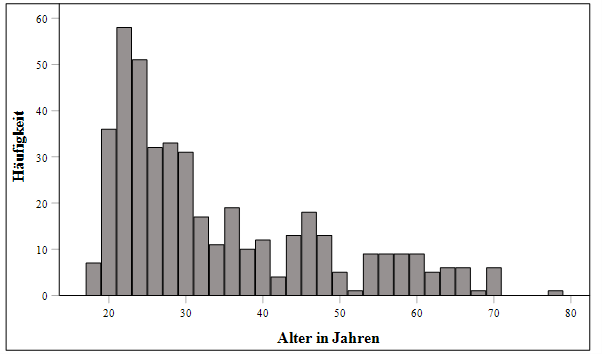
\includegraphics[width=0.8\linewidth]{Histogramm - Altersverteilung.png}
        \caption[Histogramm Altersverteilung]{Histogramm für die Altersverteilung.}
        \label{Histogramm Altersverteilung}
\end{figure}


Mit $n = 305$ (70.60\%) bilden weibliche Teilnehmer den größten Teil der Gesamtstichprobe ab. Männliche Teilnehmer betrugen 28.9\% ($n = 125$) der Befragten. Des Weiteren gaben 0.5\% ($n = 2$) der Probanden an ein diverses Geschlecht zu haben. Das Durchschnittsalter der Teilnehmer lag bei $M = 33.52$ Jahren ($SD = 13.67$). Eine grafische Darstellung der Altersverteilung ist in Abbildung~\ref{Histogramm Altersverteilung} zu sehen. An ihr lässt sich ablesen, dass der jüngste Teilnehmer 18 Jahre alt war, der älteste betrug ein Alter von 77 Jahren. Es handelt sich dabei um eine unimodale und rechtsschiefe verteilung. 



\section{Untersuchungsdesign}  \label{sec_3.2}
Die vorliegende Studie ist Teil eines größeren Forschungsprojektes, das weitere vier Arbeiten, mit ihren jeweiligen Schwerpunkten, beinhaltet. Jede dieser Arbeiten beschäftigte sich mit den Themen der häuslichen Gewalt und das der Gewaltmythen. Das Gesamtprojekt wurde der Ethikkommision vorgelegt und wurde präregistriert. Bevor der Fragebogen zur Erhebung freigegeben werden konnte, lief er einen Pretest vom 30.05.2022 bis 02.06.2022 durch. So konnten mögliche Fehler und Probleme behoben werden, um eine gute Durchführung für die Teilnehmer zu gewährleisten.

Vorraussetzung für die Teilhabe an der Umfrage waren ein internetfähiges Endgerät, die Erreichte Volljährigkeit und eine ausreichende Beherrschung der deutschen Sprache. 

Für die Datengeneration wurde ein Onlinefragbogen erstellt, da dadurch eine weitreichendere und ökonomischere Erhebung gewährleistet werden konnte. Auf diese weise konnnten der Interview- und der Versuchsleitereffekt vermieden werden. Der Zugangslink wurde primär über die sozialen Netzwerke WhatsApp, Instagram, Facebook, Telegram und Signal verschickt, weshalb es sich um eine anfallende Stichprobe handelt. 

Bezüglich der Erhebungsmethode und -Design handelt es sich bei dieser Arbeit um eine quantitative Querschnittstudie, auf der Basis eines einzigen Messzeitpunktes.
%Feld-Laborstudie\\
%effekte\\


\section{Operationalisierung der Konstrukte}    \label{sec_3.3}
Damit die Teilnehmer unvoreingenommen die, der Wahrheit ähnelten, fiktiven Fallvignetten bewerten konnten, begann der Fragebogen mit zwei zufällig zugeodneten Vignetten, die psychische oder sexualisierte Gewalt behandelten. Darauf folgte die deutsche Version der Skala zur Erfassung der Akzeptanz von Gewaltmythen. Im Anschluss befand sich eine umfangreiche Testbatterie mit vier Skalen um physische wie verbale Aggression, den Ärger und das Misstrauen zu messen. Abschließend wurden die soziodemografischen Daten wie Alter, Geschlecht, kultureller Hintergrund, Bildungsstand, berufliche Situation und das Einkommen erfragt.

Mithilfe der Fallvignetten zur häuslichen Gewalt wurde die Verantwortungszuschreibung erhoben. Insgesamt wurden 16 unterschiedliche Vignetten generiert, um vier verschiedene Variablen messen zu können. Bei diesen Variablen handelte es sich umd die Gewaltart (psychisch oder sexualisiert), das Geschlecht (männlich oder weiblich), den sozioökonomischen Status (hoch oder niedrig) und um den kulturellen Hintergrund (deutsch oder arabisch). Über einen Schiberegler konnten die Probanden die relative Verantwortung von Opfer und Täter bewerten. Die Codierung verlief vom kleinstmöglichen Punktewert auf der linken Seit bis zum größtmöglichen Punktewert auf der rechten Seite (Codierung 1-101). Eine solchen Vignette war wie folgt gegeben: %TEXT

Die Akzeptanz von häuslichen Gewaltmythen wurden mithilfe der deutschen Übersetzung des englischen Domestic Violence Myth Acceptance Scale (DVMAS) \parencite{Peters2003} unternommen. Bis auf das letzte Item sind alle übrigen 17 Items als Aussagen vormuliert und wurden mithilfe einer siebenstufigen Skala, von 1 = \enquote{Stimme überhaupt nicht zu} bis 7 = \enquote{Stimme völlig zu}, beantwortet. Ein solches Item war wie folgt: %TEXT
Für die deutsche Übersetzung des DVMAS liegt bislang noch keine Validierung vor. Da es hierbei um eine Sinngemäße Übersetzung handelt wird die Reliabilität und Validität des originalen DVMAS herangezogen. Die Reliabilität von Cronbachs-\textalpha~=~.88 liegt in einem sehr gute Bereich. Des Weiteren liegt auch eine gute Validität vor, zumal der DVMAS signifikante Korrelationen mit den folgenden vier theoretisch ähnelnden Skalen aufweist: Attitude Towards Women, Rape Myth acceptance scale, Sex Role Stereotypes und Attitude Towards Wife Abuse \parencite{DVMAS_Peters}.

Das letzte erhobene Konstrukt Aggression wurde mithilfe des Deutschen Aggressionsfragebogens erfasst. Dieser umfasst 29 Items verteilt auf den folgenden vier Subskalen: physische Aggression, verbale Aggression, Ärger und Misstrauen. Die als Aussage formulierten Items wurden anhand einer vier-stufigen Likertskala von 1 = \enquote{trifft nich zu} bis 4 = \enquote{trifft voll zu} beantwortet. Ein solches Item war wie folgt: %TEXT
Die Validität des Fragebogens wurde durch die signifikante Korrelationen mit Aggressivität, generalisierter Selbstwert, Ärger, Ärgerkontrolle und Neurotizismus festgestellt. Die Reliabilität variiert zwischen \textalpha~=~.62 und \textalpha~=~.82 (Cronbachs-\textalpha der Subskalen) und weißt eine Retestreliabilität von Cronbachs-\textalpha~=~.73\parencite{Aggressionsfragebogen}.

Die Reliabilität ist aufgrund des standatisierten Fragebogens gegeben. Es kann auch von einer gegebenen Objektivität ausgegangen werden, weil ohne einen Versuchsleiter die Probanden den Fragebogen eigenständig durchgeführten mussten. Aufgrund der Relevanz dieser Befragung ist sie valide.


%Fragestellung und Hypothesen hier dazwischen (Sophia)

\section{Untersuchungsdurchführung}   \label{sec_3.4}
Über den Zeitraum vom 04.06.2022 bis 27.06.2022 erstreckte sich die Datenerhebung. Der über SoSci-Survey erstellte Fragebogen wurde primär über den Messenger-Dienst WhatsApp, aber auch über Instagram, Facebook, Signal und Telegram verbreitet, mit der Bitte der Verbreitung, um eine möglichst große Stichprobe zu erreichen. Die Mindeststichprobengröße von 395 wurde mithilfe des kostenlosen Tools G*Power ermittelt. %G*Power (https://bjoernwalther.com/eine-kurze-einfuehrung-in-gpower/)

Im Einführungstext, zu Beginn der Befragung, wurden Auskünfte über die 15 minütige Bearbeitungszeit, wie auch die garantierte Anonymität der Probanden aufgeklärt. Die Teilnehmer wurden zudem darauf hingewiesen, dass die Teilnahme der Befragung freiwillige ist. Bevor auf die nächste Seite weitergeklickt werden konnte, wurde mithilfe einer zu beantworteten Frage sichergestellt, dass die Person den Einleitungstext verstanden hat und mit der Befragung einverstanden ist. Auf der anschließenden Seite folgte die Aufgabenerklärung für die Fallvignetten, wie eine kleine Aufklärung diesbezüglich. Jeweils nach jeder dargebotener Vignette folgten vier Fragen, zur überprüfung der Manipulation. Anschließend folgten die deutsche Übersetzung des DVMAS und der Deutsche Aggressionsfragebogen. Zum Schluss wurden die Probanden gebeten einige kurze Angaben zu ihrer Person zu geben, woraufhin eine letzte Nachfrage der gewissenhaften Durchführung folgte. Damit endete der für die Forschenden wichtige Teil der Befragung. Auf einer daran anschließenden Seite wurden Informationen und Kontaktdaten für Betroffene von häuslicher Gewalt gewährleistet. 

Mit Abschließen der befragung wurden die Probanden, die über das SONA-System kamen wieder dorthin zurückgeführt und ihnen wurden 0.25 Versuchspersonenstunden angerechnet.

Potenzielle Störvariablen konnten während der Untersuchungsdurchführung nicht kontrolliert werden. Anhand der Onlinebefragung lag die Entscheidung, zu welchem Zeitpunkt, an welchem Ort und unter welchen Bedingungen die Befragung bearbeitet wurde, bei den Teilnehmern selbst.


\section{Auswertungsmethode}    \label{sec_3.5}
Der erhobene Datensatz wurde mithilfe der Statistik- und Analysesoftware SPSS berechnet. Bevor die Hypothesen jedoch berechnet werden konnten, musste der Datensatz bereinigt werden. So, wie die Fallvignetten im Fragebogen konzipiert waren, musste der Datensatz verdoppelt werden, damit mit den Daten der Vignetten gerechnet werden konnte. 

Anschließend konnten die Daten ausgewertet werden, beginnend mit den deskriptiven Kennzahlen der drei Konstrukte. Anhand der Lageparameter, der Maße der Streuung und der Verteilung konnten die demographischen Daten der Stichprobe ausgewertet werden.

Damit die Fallvignetten wie auch der Aggressionsfragebogen für die Berechnungen genutzt werden konnten, mussten jeweils einige Items umgepolt werden. Damit bei den Vignetten den betroffenen Person stets der Zahlenwert 101 (Schieberegler rechts) zugeordnet wird, wurden jeweils bei den psychischen und sexualisierten Vignetten drei Fälle umkodiert. Ferner beinhalteten die Vignetten weitere Variablen, die für die Auswertung bei dieser Arbeit, wie auch bei den Auswertungen der weiteren Projektmitglieder wichtig waren. Für die individuelle Verwendung dieser, wurden sie aus den entsprechenden Fallvignetten extrahiert und jeweils zu einer separaten dummy-kodierten Variable dichotomisiert. Beim Aggressionsfragebogen wurden Item 14 "Ich bin eine ausgeglichene Person." und Item 22 "Ich kann mir keinen Grund vorstellen, weshalb ich jemals eine andere Person schlagen würde." umgepolt.

Die in Kapitel ~\ref{sec_3.4} bereits erwähnten Manipulationschecks wurden mithilfe des Chi$^2$-Tests berechnet.

Zur Beantwortung der ersten Hypothese (H1) wurde eine Spearman-Rang-Korrelation berechnet. Es wurde eine positive Korrelationen zwischen dem metrischen Aggressionsscore und der ordinalen Verantwortungszuschreibung auf das Opfer untersucht. Die Ordinalskalierung mindestens einer Variablen, sowie die paarweise Beobachtung sind die Vorraussetzungen für diesen Test.

Für die zweite Hypothese (H2) wurde eine Pearson-Moment-Korrelationen gerechnet, um die positive Korrelationen des metrischen Aggressionsscores mit der metrischen Akzeptanz von Gewaltmythen untersucht. Voraussetzungen für diesen Test sind, die Intervallskalierung oder Dichotomie beider Variablen, eine bestehende Linearität, die Abwesenheit von Ausreißern, sowie die Endlichkeit der Varianz bzw. Kovarianz.

Bei der dritten Hypothese (H3) handelte es sich um eine Moderationsanalyse, die mithilfe des Plug-in PROCESS berechnet wurde. Untersucht wurde bei dieser Hypothese ob das Geschlecht den Zusammenhang zwischen Akzeptanz von Gewaltmythen und Aggression moderiert. Die allgemeinen Vorraussetzung für diesen Test sind die Linearität und der Stichprobenumfang. Des Weiteren gibt es spezifische Voraussetzungen. Eine gegebene Homoskedastizität, Normalverteilung des Fehlers, keine Autokorrelation und keine Multikolinearität müssen gegeben sein.
\chapter{Ergebnisse}   \label{ch_4}
Im folgenden Kapitel werden die durchgeführten statistischen Berechnungen dargestellt. Zu Beginn werden die deskriptiven Ergebnisse beschrieben und mit den Normwerten verglichen, woraufhin die statistische Überprüfung der Manipulation folgt. Im inferenzstatistischen Unterkapitel wird mit der Prüfung der Vorraussetzung der einzelnen Test mathematisch dargestellt und abschließend werden die Ergebnisse der drei Hypothesen präsentiert. Die ausführliche Interpretation der Ergebnisse geschieht im nachkommenden Kapitel ~\ref{ch_5}. 
Wie zuvor erklärt, musste der Datensatz verdoppelt werden, um eine Berechnung mit den Daten gewährleisten zu können. Aus diesem Grund wird in diesem und den nachfolgenden Kapiteln von einer Stichprobengröße von $N_{neu}$~=~864 ausgegangen.

\section{Deskriptive Ergebnisse}    \label{sec_4.1}
Die Fallvignetten wießen, bei einem $Min$~=~1 und einem $Max$~=~101, einen Mittelwert von $M$~=~26.46 ($SD$~=~27.98) auf. Der Median lag bei $Mdn$~=~19. Die am häufigsten verteilten Werte liegen an den beiden Extremen bei 1.00 und 101.00 und bilden eine bimodale Verteilung. Bei einer Schiefe von 1.17 und Kurtosis von 0.53, liegt eine rechstschiefe beziehungsweise. linkssteile und steilgipflige Verteilung vor. Abbildung~\ref{Histogramm VicBlame} stellt die unimodale Verteilung der Verantwortungszuschreibung bildlich da. Die vorhandenen Ausreißer befinden sich alle unter der Ausscheidungsgrenze.
% Modus: 1.00 und 101.00
\begin{figure}[htb]
    \centering
        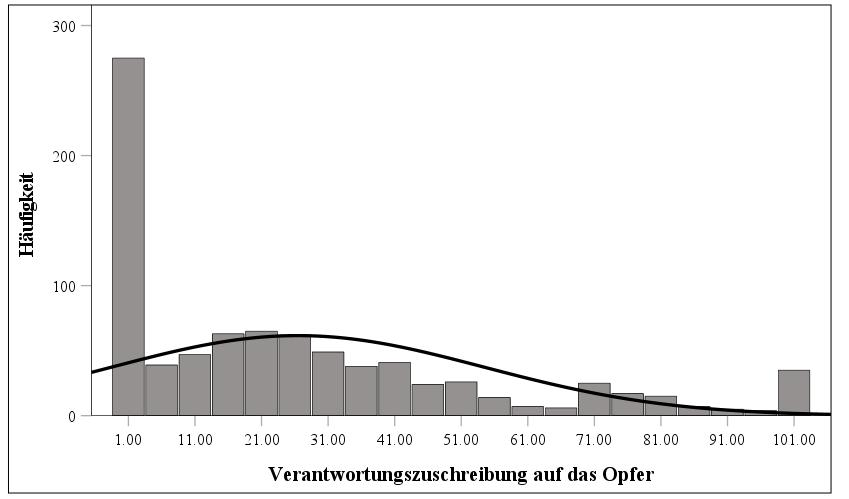
\includegraphics[width=0.8\linewidth]{Histogramm VicBlame.jpg}
        \caption[Histogramm Verantwortungszuschreibung]{Verteilung der Verantwortungszuschreibung.}
        \label{Histogramm VicBlame}
\end{figure}



Der DVMAS zeigte einen Mittelwert von $M$~=~2.60 ($SD$~=~0.80) und einen Median von $Mdn$~=~2.5. Der geringste Wert war dabei $Min$~=~1 und der höchsete $Max$~=~5.56. Die häufigsten Werte lagen bei 2.11 und 2.67 und bilden eine bimodale Verteilung. Eine Schiefe von 0.60 bildet eine leicht rechstschiefe Verteilung. Die Kurtosis von 0.09 bildet eine leicht steilere Verteilung, als die Normalverteilung. Beide Werte weichen demzufolge leicht von einer Normalverteilung ab ($M$~=~2.30, $SD$~=~0.85 und Schiefe~=~0.63). 
Die Abbildung~\ref{Histogramm DVMAS} bildet die beschriebenen Werte dieser Studie bildlich ab. Die vorhandenen Ausreißer befinden sich alle unter der Ausscheidungsgrenze.
% Modus: 2.11, 2.67
\begin{figure}[htb]
    \centering
        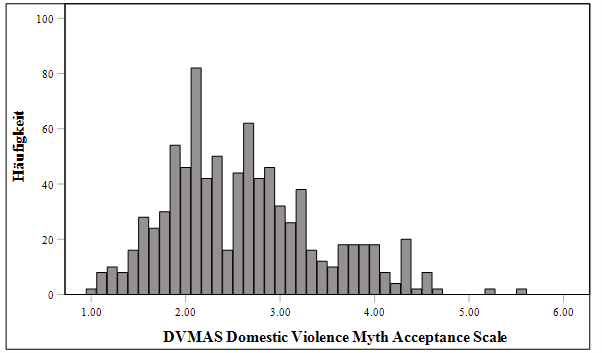
\includegraphics[width=0.8\linewidth]{Histogramm - DVMAS.png}
        \caption[Histogramm Altersverteilung]{Verteilung der Akzeptanz von Gewaltmythen.}
        \label{Histogramm DVMAS}
\end{figure}



\begin{figure}[htb!]
    \centering
        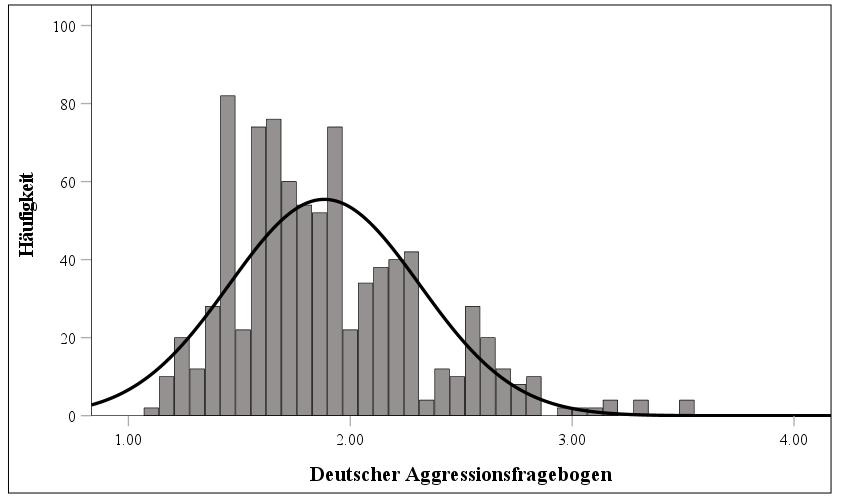
\includegraphics[width=0.8\linewidth]{Histogramm AggroFB.jpg}
        \caption[Histogramm Aggressionsfragebogen]{Verteilung der Angaben des Aggressionsfragebogens.}
        \label{Histogramm AggroFB}
\end{figure}


Beim Deutschen Aggressionsfragebogen wurde ein Mittelwert von $M$~=~1.88 ($SD$~=~0.43) und ein Median von $Mdn$~=~1.79 berechnet. Der geringste angegebene Wert betrug $Min$~=~1.10 und der höchste $Max$~=~3.52. Die Verteilung wies einen Schiefe von 0.94 und eine Kurtosis von 0.88 auf. Demzufolge ist die Verteilung rechstschiefe und hat eine breitgipflige Form, sowie eine Multimodalität mit den Modiwerten bei 1.59, 1.62, 2.52 und 2.55. Die Lageparameter weichen stark von den Normwerten ab. Diese sind wie folgt: $M$~=~2.66 ($SD$~=~0.88), Schiefe~=~3.81 und eine Kurtosis von -0.06. In Abbildung~\ref{Histogramm AggroFB} ist eine bildliche Darstellung der erhobenen Verteilung zu sehen. Die vorhandenen Ausreißer befinden sich alle unter der Ausscheidungsgrenze.
% Modus: 1.59, 1.62, 2.52, 2.55


\section{Inferenzstatistische Ergebnisse}    \label{sec_4.2}
Anschließend erfolgt eine inferenzstatistische Analyse der erhobenen Daten zur Fesstellung der Korrelationen zwischen den in Kapitel~\ref{ch_2} näher gebrachten Konstrukte Aggression, Akzeptanz der Gewaltmythen und die Verantwortungszuschreibung. 


\subsection{Hypothese 1}    \label{subsec_4.2.1}
Die Hypothese 1 geht von einer Korrelation des Aggressionsscores mit Victim Blaming aus. Diese ungerichtete Zusammenhangshypothese wurde mit der Spearman$-$Rang$-$Korrelation berechnet. Die in Kapitel ~\ref{sec_3.5} erwähnten Voraussetzungen der Ordinalität beider Variablen wie auch die paarweise Beobachtungen sind gegeben. Eine gepaarte Beobachtung entspricht einer gemessenen Variable pro Spalte bei SPSS.
\begin{table}[htb]
    \caption[Mittelwerte, Standardabweichung und Korrelation von Aggression und Victim Blaming]{\textit {Mittelwerte, Standardabweichung und Korrelation von Aggression und Victim Blaming}} 
    \label{H1_Spearman}
    \centering
    \begin{adjustbox}{width=6.5cm} %{maxwidth=\textwidth}
    \small
    \begin{tabular}{lrrr}
      \hline
        & $M$   & $SD$ & 1 \\
      \hline
    1 Aggression      & 1.88  & 0.43   & $-$      \\
    2 Victim Blaming  & 26.46 & 27.98  & .18      \\
       \hline
    \end{tabular}
    \end{adjustbox}
    
    \begin{tablenotes}
        \item \textit{Anmerkungen.} \( N_{neu} \)~=~864; Wertebereich der Variable Aggression 1 (\textit{trifft nicht zu}) bis 4 (\textit{trifft voll zu}); Spearman$-$Rang$-$Korrelation.
      \end{tablenotes}
    \end{table}



Das in Tabelle~\ref{H1_Spearman} ersichtliche Ergebnis der Spearman$-$Rang$-$Korrelation fiel nicht signifikant aus ($p$~=~n.s.). Mit dem sehr kleinen Effekt \parencite{Cohen_1992} von $r_{s}$~=~.18, korreliert die Aggression nur sehr gering mit der Verantwortungszuschreibung auf das Opfer.

\subsection{Hypothese 2}    \label{subsec_4.2.2}
Die Voraussetzung einer Pearson$-$Produkt$-$Moment$-$Korrelation wurden in ~\ref{sec_3.5} bereits aufgeführt. In diesem Falle sind auch alle Voraussetzungen gegeben: Aggression und die Akzeptanz von Gewaltmythen sind metrisch, die vorhandenen Ausreißer sind im akzeptablen Bereich (siehe Anhang~\ref{Boxplot_AggroFB} und Anhang~\ref{Boxplot_DVMAS}), 
es liegt ein linearer Zusamenhang zwischen den Variablen vor (siehe Anhang~\ref{Linearitat_AggroFB_DVMAS}) und eine bivariate Normalverteilung ist auch gegeben, da der Bootstrap$-$Konfidenzintervall (.308 $-$ .442) die Null nicht einbezieht.

Die in Tabelle~\ref{H2_Pearson} ersichtliche Pearson$-$Produkt$-$Moment$-$Korrelation zeigte einen Zusammenhang von $r$~=~.38. Nach \textcite{Cohen_1992} entspricht dies einer mittelgroßen Korrelation, die bei einseitiger Testung statistisch signifikant ausfiel ($p<$ .001).
\begin{table}[htb]
    \caption[Mittelwerte, Standardabweichung und Korrelation von Aggression und der Akzeptanz von Gewaltmythen]{\textit {Mittelwerte, Standardabweichung und Korrelation von Aggression und der Akzeptanz von Gewaltmythen}} 
    \label{H2_Pearson}
    \centering
    \begin{adjustbox}{width=5.5cm} %{maxwidth=\textwidth}
    \small
    \begin{tabular}{lrrr}
      \hline
        & $M$   & $SD$ & 1 \\
      \hline
    1 Aggression      & 1.88 & 0.43  & $-$      \\
    2 DVMAS           & 2.60 & 0.80  & .38*      \\
       \hline
    \end{tabular}
    \end{adjustbox}
    
    \begin{tablenotes}
        \item \textit{Anmerkungen.} \( N_{neu} \)~=~864; DVMAS = Akzeptanz der Gewaltmythen; Wertebereich der Variable Aggression 1 (\textit{trifft nicht zu}) bis 4 (\textit{trifft voll zu}); Variable DVMAS 1 (stimme überhaupt nich zu) bis 7 (stimme völlig zu); Pearson$-$Produkt$-$Moment$-$Korrelation. \\ *$p<$~.001
      \end{tablenotes}
    \end{table}




\subsection{Hypothese 3}    \label{subsec_4.2.3}
Um die vermutete Moderation des biologischen Geschelchts auf den Zusammenhang zwischen Aggressio und dem DVMAS zu testen, wurde eine Moderationsanalyse durchgeführt. Die Variablen weisen eine lineare Beziehung und eine Unabhängigkeit, durch die nicht verbundene Erhebung der einzelnen Variablen, auf. Durch die mit $N_{neu}$~=~864 großen Stichprobe, kann von einer Normalverteilung der Residuen ausgegangen werden. Die Überprüfung der Homoskedastizität mithilfe des White$-$Tests ergab eine signifikantes Ergebnis ($p$~=~.03). Somit liegt eine Heteroskedastizität vor. 

\begin{table}[htb]
    \caption[Moderationsanalyse Geschlecht und Aggression auf die Akzeptanz von Gewaltmythen]{\textit {Moderationsanalyse Geschlecht und Aggression auf die Akzeptanz von Gewaltmythen}} 
    \label{Moderationsanalyse}
    \centering
    \begin{adjustbox}{width=11cm} %{width=\textwidth}
    \small
    \begin{tabular}{lrrrrr}
      \hline
      & $B$    & $SE(B)$  & $t$    & $p$ & $\Delta R^{2}$\\
      \hline
    Konstante  & 2.59    & 0.03 & 103.13  & $<$~.001 & \\
    Aggression & 0.68    & 0.06 & 11.13   & $<$~.001 & \\
    Geschlecht & $-$0.24 & 0.05 & $-$4.32 & $<$~.001 & \\
    Interaktionsterm & $-$0.14 & 0.13 & $-$1.06 & .290 & .001 \\
    $R^{2}$          &         &      &         &      & .163* \\
       \hline
    \end{tabular}
    \end{adjustbox}
    
    \begin{tablenotes}
        \item \textit{Anmerkungen.} \( N_{neu} \)~=~864; *$p<$~.001
      \end{tablenotes}
    \end{table}




Das Gesamtmodell war, wie in Tabelle~\ref{Moderationsanalyse} demonstriert, mit einer Varianzaufklärung von 16.34\% signifikant ($F$(3, 856)~=~50.30, $p<$ .001). Die Moderationsanalyse konnte jedoch keinen signifikanten Moderationseffekt finden, $\Delta R^{2}$~=~0.12\%, F(1, 860)~=~1.12, $p$~=~.290, 95\% CI[-0.39, 0.12]. Dennoch klärt das Modell 16.34\% der Varianz des deutschen DVMAS auf.
%Modell: $R^{2}$~=~16.34\%, $F$(HC3)~=~50.30, $df1$~=~1, $df2$~=~856 $p<$~.001
%W*X: $\Delta R^{2}$~=~0.08, $F$(HC3)~=~0.76, $df1$~=~1, $df2$~=~856 $p$~=~.384

\begin{table}[htb]
    \caption[Modell mit Haupteffekten]{\textit {Modell mit Haupteffekten}} 
    \label{Haupteffekte}
    \centering
    \begin{adjustbox}{width=10.5cm} %{width=\textwidth}
    \small
    \begin{tabular}{lrrrrr}
      \hline
               & $B$    & $SE(B)$ & \textbeta  & $t$    & $p$ \\
      \hline
    Geschecht  & $-$.23 & 0.06    & $-$.13   & 4.191  & $<$~.001 \\
    Aggression & .69    & 0.06    & .37      & 11.842 & $<$~.001 \\
       \hline
    \end{tabular}
    \end{adjustbox}
    
    \begin{tablenotes}
        \item \textit{Anmerkungen.} \( N \) = 864%; *$p<$~.001
      \end{tablenotes}
    \end{table}


Den Entfehlungen von \textcite{Moderation_SPSS} folgend, wurde der Interaktionsterm herausgenommen. Dies führte zu einem neuen Modell mit Haupteffekten, welche in Tabelle~\ref{Haupteffekte} zusammengefasst wurden. Die Beziehung zwischen Geschlecht ($B$~=~$-$.23, $p<$~.001), wie auch zwische Aggression ($B$~=~.69, $p<$~.001) und der Akzeptanz von Gewaltmythen fiel signifikant aus. 
%Geschlecht: $B$~=~$-$.23, $(SE)B$~=~0.06, $\beta$~=~$-$.13, $t$~=~$-$4.191, $p<$~.001
%Aggression: $B$~=~.69, $(SE)B$~=~0.06, $\beta$~=~.37, $t$~=~11.842, $p<$~.001


\section{Manipulationscheck}    \label{sec_4.3}
Nachfolgend werden die Ergebnisse der vier Manipulationschecks in der folgenden Reihenfolge aufgeführt: Gewaltart, Geschlecht des Opfers, soziökonomischer Status der betroffenen Person und abschließend der Kulturelle Hintergrund.


\begin{table}[htb]
    \caption[Kreuztabelle Manipulationscheck Gewaltart]{\textit {Kreuztabelle des Manipulationschecks der Gewaltart}} 
    \label{KT_G}
    \centering
    \begin{adjustbox}{width=10cm} %{width=\textwidth}
    \small
    \begin{tabular}{lrrr}
      \hline
        &   & psychische Gewalt & sexualisierte Gewalt \\
      \hline
    Ja   & Anzahl  & 32      & 354     \\
         & Prozent & 8.30\%  & 91.70\% \\
    Nein & Anzahl  & 400     & 78      \\
         & Prozent & 83.70\% & 16.30\% \\
       \hline
    \end{tabular}
    \end{adjustbox}
    
    \begin{tablenotes}
        \item \textit{Anmerkungen.} \( N \) = 864. Prüffrage: Ging es um sexualisierte Gewalt?
      \end{tablenotes}
    \end{table}
\begin{table}[htb]
    \caption[Kreuztabelle Manipulationscheck Opfergeschlecht]{\textit {Kreuztabelle des Manipulationschecks des Geschlecht der betroffenen Person}} 
    \label{KT_sex}
    \centering
    \begin{adjustbox}{width=\textwidth}
    \small
    \begin{tabular}{lrrr}
      \hline
        &   & weibliches Opfer & männliches Opfer \\
      \hline
    Ja   & Anzahl  & 411      & 14      \\
         & Prozent & 96.70\%  & 3.30\%  \\
    Nein & Anzahl  & 16       & 423     \\
         & Prozent & 3.60\%   & 96.40\% \\
       \hline
    \end{tabular}
    \end{adjustbox}
    
    \begin{tablenotes}
        \item \textit{Anmerkungen.} \( N \) = 864. Prüffrage: War das Opfer eine Frau?
      \end{tablenotes}
    \end{table}
Bei der Überprüfung der Gewaltart gaben bei Vignetten sexualisierter Gewalt 354 Personen (91.70\%) an eine solche Gewaltart behandelt zu haben. Handelte es sich um eine psychische Gewaltart an, reichten nur 400 Personen (83.70\%) die richtige Antwort ein. Der durchgeführte Chi$^2$-Test viel mit einem Wert von 485.53 signifikant aus ($p<$.001). 
In Tabelle~\ref{KT_G} sind die Werte dieser Manipulationsprüfung nochmals zusammengefasst.

War die Nachfrage auf das Geschlecht des Opfers gerichtet gaben die 411 (96.70\%) bzw. 423 (96.40\%) Probanden an, es handelte sich um ein weibliches bzw. männliches Opfer. Auch dieser Chi$^2$-Test war mit einem Wert von 748.16 hoch signifikant ($p<$.001). 
In Tabelle~\ref{KT_sex} sind die Werte dieser Manipulationsprüfung nochmals zusammengefasst.

Die Überprüfung des niedrigen soziökonomischen Status des Opfers wurde von 389 (80.2\%) bei dessen Gegebenheit richtig beanwortet. Bei der gegenteiligen Situation stieg die Rate der richtigen Antworten auf 342 (90.20\%). Mit einem Wert von 422.37 fiel dieser Chi$^2$-Test ebenfalls signifikant aus ($p<$.001). 
In Tabelle~\ref{KT_SES} sind die Werte dieser Manipulationsprüfung nochmals zusammengefasst.
\begin{table}[htb]
    \caption[Kreuztabelle Manipulationscheck soziökonomischer Status des Opfers]{\textit {Kreuztabelle des Manipulationschecks des soziökonomischen Status der betroffenen Person}} 
    \label{KT_SES}
    \centering
    \begin{adjustbox}{width=10cm} %{width=\textwidth}
    \small
    \begin{tabular}{lrrr}
      \hline
        &   & niedriger SES Opfer & hoher SES Opfer \\
      \hline
    Ja   & Anzahl  & 389      & 96      \\
         & Prozent & 80.20\%  & 19.8\%  \\
    Nein & Anzahl  & 37       & 342     \\
         & Prozent & 9.80\%   & 90.20\% \\
       \hline
    \end{tabular}
    \end{adjustbox}
    
    \begin{tablenotes}
        \item \textit{Anmerkungen.} \( N_{neu} \)~=~864. SES = soziökonomischer Status. Prüffrage: War die finanzielle Situation des Opfers schlechter als die finanzielle Situation des Täters?
      \end{tablenotes}
    \end{table}

\begin{table}[htb]
    \caption[Kreuztabelle Manipulationscheck kultureller Status]{\textit {Kreuztabelle des Manipulationschecks des kulturellen Status}} 
    \label{KT_kult}
    \centering
    \begin{adjustbox}{width=6.5cm} %{width=\textwidth}
    \small
    \begin{tabular}{lrrr}
      \hline
        &   & arabisch & deutsch \\
      \hline
    Ja   & Anzahl  & 10      & 422      \\
         & Prozent & 2.30\%  & 97.70\%  \\
    Nein & Anzahl  & 423     & 9        \\
         & Prozent & 97.90\% & 2.10\%   \\
       \hline
    \end{tabular}
    \end{adjustbox}
    
    \begin{tablenotes}
        \item \textit{Anmerkungen.} \( N_{neu} \)~=~864. Prüffrage: Hatten die Personen deutsche Namen?
      \end{tablenotes}
    \end{table}
Die höchste Rate an Richtigkeit gab es bei dem Manipulationscheck des kulturellen Status. Hier gaben 422 (97.70\%) Personen bzw. 423 (97.90\%) die richtige Antwort. Auch dieser Chi$^2$-Test ist mit einem Wert von 789.68 signifikant ($p<$.001). 
In Tabelle~\ref{KT_kult} sind die Werte dieser Manipulationsprüfung nochmals zusammengefasst.

Bei der Kontrollfrage gaben zwei Personen an, nicht sinnvolle Angaben hinterlegt zu haben. Da es statistisch keinen unterschied gibt, ob sie ausgeschlossen werden oder nicht, verblieben sie im Datensatz.


\section{Explorative Ergebnisse}    \label{sec_4.4}
Zusätzlich zu den untersuchten Hypothesen wurden noch weitere explorative Untersuchungen getätigt. In Kapitel~\ref{subsec_4.4.1} wurde getestet, ob die Subskalen von Aggression positiv untereinander und mit dem DVMAS korreliert. 

%Des Weiteren wurde Aggression mit dem kultuerllen Hintergrund der Probanden (vgl. Kapitel~\ref{subsec_4.4.2}) korreliert. Der Deutsche Aggressionsfragebogen unterlief zwei Unterschiedtestungen. In Kapitel~\ref{subsec_4.4.3} wurde exploriert, ob sich die Aggressionsausprägung zwischen den kulturellen Hintergründen unterscheidet und in Kapitel~\ref{subsec_4.4.4} mit den biologischen Geschlechtern der Probanden.


\subsection{Korrelation Aggresion-Subskalen mit DVMAS}  \label{subsec_4.4.1}
\begin{table}[htb]
    \caption[Mittelwerte, Standardabweichung und Korrelation der Aggression$-$Subskalen, DVMAS und Victim Blaming]{\textit {Mittelwerte, Standardabweichung und Korrelation der Aggression$-$Subskalen, DVMAS und Victim Blaming}} 
    \label{lala}
    \centering
    \begin{adjustbox}{width=14cm} %{width=\textwidth}
    \small
    \begin{tabular}{lrrrrrrrr}
      \hline
        Variablen             & $M$  & $SD$   & 1     & 2     & 3     & 4    & 5 & 6\\
       \hline
       1 physische Aggression & 1.60  & 0.55  &       &       &        &      & &\\
       2 verbale Aggression   & 2.22  & 0.53  & .36** &       &        &      & &\\
       3 Ärger                & 1.96  & 0.58  & .46** & .39** &        &      & &\\
       4 Misstrauen           & 1.93  & 0.60  & .31** & .27** & .45**  &      & &\\
       5 DVMAS                & 2.60  & 0.80  & .28** & .25** & .19**  & .24** & &\\
       6 Victim Blaming       & 26.58 & 27.99 & .07*  & .02   & .04    & .02   & & \\
    \end{tabular}
    \end{adjustbox}
    
    \begin{tablenotes}
        \item \textit{Anmerkungen.} \( N_{neu} \)~=~864; DVMAS = Akzeptanz der Gewaltmythen; Wertebereich der Aggression-Subskalen von 1 (\textit{trifft nicht zu}) bis 4 (\textit{trifft voll zu});  DVMAS von 1 (\textit{stimme überhaupt nicht zu}) bis 7 (\textit{stimme völlig zu}); Victim Blaming von 1 (\textit{Verantwortungszuschreibung auf den Täter}) bis 101 (\textit{Verantwortungszuschreibung auf das Opfer}); Spearman$-$Rang$-$Korrelation. *$p<$~.05, **$p<$~.001
      \end{tablenotes}
    \end{table}



Für die Korrelation zwischen den drei Aggressions-Subskalen verbale Aggression, Ärger und Misstrauen und der Akzeptanz von Gewaltmythen wurde eine Pearson$-$Produkt$-$Moment$-$Korrelation berechnet, denn alle Variablen sind metrisch skaliert. Des Weiteren ist die Linearität zwischen den Variablen gegeben. Da die Variable der physischen Aggression zu große Ausreißer aufwies, wurde sie aus der Korrelationsrechnung ausgeschlossen. Auch eine bivariate Normalverteilung ist bei den verbliebenen Korrelation vorhanden und lauten wie folgt: verbale Aggression$-$Ärger CI [0.39, 0.51], verbale Aggression$-$Misstrauen CI [0.23, 0.36], verbale Aggression$-$DVMAS CI [0.20, 0.34], Ärger$-$DVMAS CI [0.18, 0.31], Misstrauen$-$DVMAS CI [0.18, 0.29], Misstrauen$-$Ärger CI [0.41, 0.53]. An den kursiv gesetzten $r-$Werte, in Tabelle~\ref{lala}, ist erkennbar, dass alle Subskalen unter sich signifikant sind und, dass sie jeweils mit dem DVMAS positiv korrelieren. 

Die verbale Aggression korrelierte mittelgradig mit Ärger ($r$~=~.45, $p<$~.001) und Misstrauen ($r$~=~.30, $p<$~.001).
Die Subskala Ärger wies eine mittelgradig Korrelation mit Misstrauen ($r$~=~.48, $p<$~.001) auf.

Der DVMAS wies bei den drei Subskalen verbale Aggression ($r$~=~.27, $p<$~.001), Ärger ($r$~=~.25, $p<$~.001) und Misstrauen ($r$~=~.24, $p<$~.001) jeweils eine schwache Korrelation auf.

%\subsection{Korrelation Aggresion-Subskalen mit Geschlecht der Probanden}   \label{subsec_4.4.2}
%Für die Korrelation zwischen Aggression und dem biologischen Geschlecht der Probanden wurde eine Spearman$-$Rang$-$Korrelation berechnet, da beide Variablen metrisch skaliert sind. An den, in %Tabelle~\ref{}, kursiv gesetzten $r-$Werte ist erkennbar, dass Aggression und der kulturelle Hintergrund negativ korrelieren. Mit $r$~=~$-$.26 bildet diese mittelgradige negative Korrelation zwischen den beiden Variablen ein signifikantes Ergebnis ($p<$~.001).   
% Die Variable des Victim Blaming ist in diesem Fall ordinal skaliert und somit ist diese Voraussetzung erfüllt. Auch die weitere Voraussetzung der paarweisen Beobachtung ist gegeben, da in SPSS eine Zeile die Erhebung einer Person darstellt. 
%     5 Geschlecht          & 1.71 & 0.45  & $-$.16** & .07* &.09** & $-$ & $-$\\
%Ein Test auf die Unterscheidung zwischen den Geschlechtern konnte nicht durchgeführt werden, da Heteroskedastizität vorlag und es so zu einem Fehler 1. Art kommen könnte.     so wie bei Kultur

%\subsection{Unterscheidung Aggression mit Geschlecht der Probanden}   \label{subsec_4.4.4}
%Auch die explorative Untersuchung der Differenz zwischen den biologischen Geschlechtern in Anbetracht der Aggression, wurde mithilfe des t-Tests für unabhängige Stichproben getestet. Der Levene Test fiel mit $F$~5.72 signifikant aus.
%Der Unterschied zwischen Männern und Frauen war signifikant ($t$(433.64)~=~2.18, $p$~=~.0.30). Die Aggression war bei Frauen durchschnittlich 0.07 Einhaeiten niedriger (95\%$-$CI[0.01, 0.14]).

\chapter{Diskussion}   \label{ch_5}
Das abschließende Diskussionskapitel beginnt mit einer Zusammenfassung der zentralen Ergebnisse. Daraufhin folgt ihre Interpretation und die Einordnung in den aktuellen wissenschaftlichen Forschungsstand. Nachfolgend werden die verwendeten Methoden bewertet. Die Arbeit endet mit theoretischen und oder praktischen Implikationen für die zukünftige Forschung oder Praxis.


\section{Zusammenfassung der zentralen Ergebnisse}  \label{sec_5.1}
Diese Bachelorarbeit befasst sich maßgeblich mit den Themen häusliche Gewalt, Gewaltmythen und deren Zusammenhang mit der Aggressivität der Probanden. Im laufe dieses Kapitels werden die Ergebnisse von den zuvor aufgestellten Hypothesen zusammgefasst sowie die Ergebnisse der Post$-$hoc Analyse.

An dem online erhobenen Fragebogen nahmen hauptsächlich junge Personen teil und mehr als die Hälfte der $N$~=~432 großen Stichprobe waren Frauen. 
Die Ergebnisse der Manipulationschecks zeigten, dass mehr als 80\% der Probanden die Vignetten richtig gelesen und verstanden haben. Auffalend war die hohe Rate an richtigen Antworten bei der Nachfrage nach dem Opfergeschlecht sowie dem kulturellen Hintergrund im Verhältnis zur Antwortrate bezüglich der Gewaltart und dem sozioökonomischen Status.


% H1: Der Aggressionsscore korreliert mit victim blaming.
Die H1 diente der Überprüfung einer möglichen Korrelation zwischen der Aggression und der Verantwortungszuschreibung auf das Opfer. Obwohl die Verteilung der Variable der Verantwortungszuschreibung nicht einer Normalverteilung entsprach, konnte sie wegen der, mit $N_{neu}$~=~864, großen Stichprobe und des zentralen Grenzwertsatzes als metrisch eingestuft werden. 
Bei der Testung der Voraussetzungen für eine Pearson$-$Produkt$-$Moment$-$Korrelation kam eine nicht bivariate Normalverteilung heraus. Aus diesem Grund wurde auf die Spearman$-$Rang$-$Korrelation ausgewichen. Für diesen Test waren alle Voraussetzungen erfüllt. Die Spearman$-$Rang$-$Korrelation ergab ein nicht signifikantes Ergebnis und auch der vorhandene Effekt war gering. Demzufolge wurde die Nullhypothese angenommen und die Aggression der Probanden korrelierte nur bedingt und nicht signifikant mit der Verantwortungszuschreibung auf das Opfer.

% H2: Der Aggressionsscore korreliert mit victim blaming.
Bei der H2 wurde eine positive Korrelation zwischen Aggression und der Akzeptanz der Mythen häuslicher Gewalt untersucht. Für dessen Überprüfung waren die Voraussetzungen der Pearson$-$Produkt$-$Moment$-$Korrelation alle gegeben. Somit konnte sie gerechnet werden. Die Testung kam zu einem signifikanten Ergebnis und einem mittelgroßen Effekt. Die Nullhypothese musste demzufolge verworfen und die Alternativhypothese angenommen werden. Die Aggression und die Akzeptanz der Gewaltmythen wiesen eine mittelsrarke Korrelation auf.

% H3: Der Zusammenhang zwischen Akzeptanz der Mythen häuslicher Gewalt und Aggression wird durch das Geschlecht moderiert.
Von einer moderierenden Rolle des biologischen Geschlechts des Probanden auf den Zusammenhang zwischen Aggression und der Akzeptanz der Mythen häuslichen Gewalt, wurde bei der H3 ausgegangen. Bei der Überprüfung der Voraussetzungen kam der White-Test zu einem signifikanten Ergebnis, was für eine Heteroskedastizität spricht. Die weiteren Voraussetzungen waren gegeben. Das Gesamtmodell der Moderation war signifikant, jedoch zeigte die Interaktion der drei Variablen ein nicht signifikantes Ergebnis. Die Nullhypothese musste demzufolge angenommen werden. Das Geschlecht hatte keine moderierende Auswirkung auf den Zusammenhang von Aggression und der Akzeptanz der Gewaltmythen. Des Weiteren wurde überprüft, ob die beiden Prädiktoren Einfluss auf das Kriterium haben. Die Regressionsanalyse zeigte für das Geschlecht und die Aggression ein signifikantes Ergebnis. Beide Variablen beeinflussten demzufolge die Akzeptanz der Mythen häuslicher Gewalt.

% explorative Ergebnisse
Die Post$-$hoc Analysen diente der weiteren Untersuchung der Korrelation von Aggression, der Verantwortungszuschreibung und der Akzeptanz der Mythen häuslicher Gewalt. Die Analyse erforschte die Korrelation zwischen den Aggression$-$Subskalen physische Aggression, verbale Aggression, Ärger und Misstrauen untereinander und jeweils mit dem DVMAS und Victim Blaming. Sie kam mit erfüllten Voraussetzungen zu signifikanten Ergebnissen. Die vier Subskalen korrelierten signifikant und mit einem mittelgroßen Effekt untereinander und mit einem schwachen Effekt mit der DVMAS. Alle vier Subskalen wiesen schwache Korrelation mit der Verantwortungszuschreibung auf das Opfer auf. Es zeigte sich, dass ausschließlich die physische Aggression signifikant mit der Verantwortungszuschreibung auf das Opfer korreliert.


\section{Einordnung und Diskussion der Befunde}     \label{sec_5.2}
Im folgenden Unterkapitel werden die Ergebnisse der Hypothesen und auch die der Post$-$hoc Analysen interpretiert, disskutiert und in den aktuellen Forschungsstand eingeordnet.

% H1:
Die H1 zeigte ein nicht signifikantes Ergebnis. Die Aggression korreliert nicht mit Victim Blaming. Dieses Ergebnis deckt sich mit dem Befund von \textcite{H1_moderation_2020}. Das vorliegende nicht signifikante Ergebnis kann möglicherweise auf die bimodale Verteilung zurückgeführt werden. Wie in Abbildung~\ref{Histogramm VicBlame} ersichtlich, gaben sehr viele Probanden dem Täter, auf der linken Seite, die Veranwortung. Auf der rechten Seite, beim Opfer, ist eine weitere vergrößerte Anhäufung der Verantwortungszuschreibung zu sehen. Gegebenenfalls waren die Vignetten zu polarisierend formuliert, oder beinhalteten zu wenige Informationen. Gemeinsam mit einer sozialen Erwünschtheit führte dies möglicherweise dazu, dass viele Teilnehmer die Veranwortung eindeutig dem Täter oder Opfer zuschrieben. Gegebenenfalls kam \textcite{H1_malasia_2012} zu einem signifikanten Ergebnis, da im Rahmen ihrer Studie Jugendliche untersucht wurden. Konträr zur Vermutung, dass durch das junge Alter vieler Probanden sich die Ergebnisse mit denen von \textcite{H1_malasia_2012} ähneln werden, gleicht sich das Ergebnis mit dem von \textcite{H1_moderation_2020}. In Kapitel~\ref{subsec_2.1.1} wurde im Sinne der positiven Aggression von dessen Nutzen im Jugendalter berichtet \parencite{Aggression}. Gegebenenfalls weisen Personen im heranwachsenden Alter ein höheres Aggressionsniveau auf, das sich bei den jungen Erwachsenen bereits verringert hat. Die Stichprobe von \textcite{H1_moderation_2020} gleicht mehr der hier Erhobenen und aus diesem Grund sind diese Ergebnisse besser vergleichbar, zumahl sie sich ähneln.

% H2:
Das signifikante Ergebnis der H2 bedeutet, dass Aggression positiv mit der Akzeptanz der Mythen häuslicher Gewalt korreliert. Obwohl bislang nicht viele Studien diese beien Konstrukte gemeinsam untersucht haben, zeigt diese Arbeit sowieauch die von \textcite{H2_u_3_Bhogal_2016, H1_moderation_2020}, dass es einen Zusammenhang gibt. Demzufolge akzeptiert eine Person mit einem höheren Aggressionsniveau vermehrt die Mythen häuslicher Gewalt. Wie bereits in Kapitel~\ref{subsec_2.1.1} vermutet, kann es daran liegen, dass die Mythen Gewalt thematisieren, die oft, wenn nicht ausschließlich, ihren Ursprung in der Aggression haben. Wie \textcite{Def_Aggressivität_vs_violence} in Kapitel~\ref{subsec_2.1.1} referenziert wurde, ist Gewalt erlerntes Verhalten, geprägt duch kulturelle Ideologien. Die gesellschaftliche Wahrnehmung und Einstellung prägen auch die Mythen häuslicher Gewalt \parencite{Labelingtheory_plus, DVMAS_Peters}. Die gesellschaftlichen und kulturellen Einstellungen und Ideologien scheinen demzufolge sowohl die Mythen sowieauch die Gewalt zu bedingen. Aus dem vorliegenden signifikanten Ergebnis lässt sich vermuten, dass diese Gewalt aus der Aggression entstammt.


% H3:
Die Moderationsanalyse der H3 zeigte eine nicht signifikante Interaktion des biologischen Geschlechts mit der Aggression und der Akzeptanz der Mythen häuslicher Gewalt. In Kapitel~\ref{subsec_2.2.3} wurde von geschlechtsspezifischen Unterschieden bezüglich der Aggressivität sowie auch der Akzeptanz der Gewaltmythen berichtet \parencite{H2_u_3_Bhogal_2016, H3_MFUnterschied, H3_2020}. Obwohl diese Studien darlegten, dass das Geschlecht sowohl auf die Aggression sowie auch auf die Akzeptanz der Mythen Auswirkungen hat, konnte diese Moderationsanalyse keinen Beleg dafür darlegen. Der Einfluss von Aggression auf die Akzeptanz der Mythen häuslicher Gewalt ist geschlechtsunabhängig. Bei der Prüfung der Voraussetzungen einer Homoskedastizität fiel der White-Test signifikan aus, das für eine Heteroskedastizität spricht. Diese kann möglicherweise zu einem nicht signifikanten Ergebnis geführt haben, obwohl beide Prädiktoren hoch signifikante Haupteffekte aufwiesen.
Der durch die Heteroskedastizität entstandene Bias des Standardfehlers kann zu fehlerhaften Interpretationen und Schlussfolgerungen des $p-$Wertes der Moderation führen \parencite{Voraussetzung_Moderation}. 

Aufgrund des dennoch nicht signifikanten Moderationseffekts, wurde eine Analyse der Haupteffekte durchgeführt. Sie zeigten einen Effekt sowohl des Geschlechts als auch der Aggression auf die Akzeptanz. Dies bedeutet, dass unabhängig voneinander das Geschlecht und die Aggression Einfluss auf die Akzeptanz der Mythen häuslicher Gewalt nehmen. Der Einfluss des Geschlechts stimmt mit den Ergebnissen von \textcite{H3_2020} überein.


%Explo
% coor subskalen dvmas
% corr subskalen vicblame
Die Spearman$-$Rang$-$Korrelationen der Post$-$hoc Analyse fiel größtenteils signifikant aus. Alle Aggression$-$Subskalen korrelierten positiv untereinander und mit der DVMAS. Nur die positive Korrelation der physischen Aggression mit der Verantwortungszuschreibung auf das Opfer fiel signifikant aus. Die weiteren Subskalen wiesen ebenfalls eine schwache positive Korrelation auf, waren jedoch nicht signifikant. Zur Untersuchung der Zusammenhänge wurde die Spearman$-$Rang$-$Korrelation verwendet, da bei der Prüfung der Voraussetzungen einer Pearson$-$Produkt$-$Moment$-$Korrelation die physische Aggression große Ausreißer aufwies. Die signifikanten Korrelation der Subskalen stimmen mit der Validierung des Deutschen Aggressionsfragebogens \parencite{Aggressionsfragebogen} überein. Somit unterstützen sie die Validität des verwendeten Fragbogens. Die signifikante positive Korrelation der Subskalen mit der DVMAS dienen einer genaueren Untersuchung der H2 Korrelation. Das Ergebnis der Korrelation der Subskalen mit Victim Blaming weicht von dem Ergebnis von \textcite{H1_moderation_2020} ab. 
% warum nur physisch signifikant?


\section{Bewertung der Methode}   \label{sec_5.3}
Dieses Unterkapitel betrachtet die verwendete Methode genauer. Es werden sowohl die Stärken sowieauch ihre Schwächen aufgewiesen.
Durch die erreichte Stichprobe von $N$~=~432 konnte die zuvor berechnete Mindeststichprobe von 395 Probanden erreicht werden. Dies ist ein Argument für eine valide Erhebung einer quantitativen Querschnittsstudie. Die Stichprobe wurde nichtrandomisiert erhoben, die sich durch den Schneeballeffekt vergrößerte.

Der Einsatz von Manipulationschecks zur Überprüfung der Verständlichkeit und bewussten Wahrnehmung der präsentierten Fallvignetten, trägt ebenfalls zu einer validen Untersuchung bei. Die Überprüfung des sozioökonomischen Status der Personen innerhalb der Fallvignetten kann zu Verwirrungen geführt haben, da gegebenenfalls von einem gemeinsamen sozioökonomischen Status des Paares ausgegangen wurde. Dennoch gewährleisten die Überprüfungen eine gute Einschätzung der Verständlichkeit der Vignetten. Dies wurde ersichtlich durch die signifikanten Ergebnisse der Chi$^2-$Tests. Das Geschlecht kann aufgrund der noch immer bestehenden Vorstellung eines überwiegend weiblichen Opfers zu dessen richtigen Identifikation geführt haben. Die ausländischen und somit, in einer deutschen Befragung, exotischeren Namen konnten der Grund für deren hohe Rate an Identifikation sein.

Der verwendete Aggressionsfragebogen sowie auch der Fragebogen zur Erfassung der Akzeptanz der Mythen häuslicher Gewalt zeigen beide eine hohe Reliabilität und Validität auf \parencite{Peters2003, Aggressionsfragebogen}. Der Aggressionsfragebogen und der deutsche DVMAS eigneten sich demzufolge gut für die Erhebung der Variablen Aggression und Akzeptanz der Gewaltmythen. 
Die Entscheidung, die Fallvignetten zu Beginn zu präsentieren, diente dazu, dass der Probanden möglichst unvoreingenommen die Verantwortung zuschreibung konnte. Diese präventive Maßnahme birgt jedoch auch Nachteile. Die Fallvignetten forderten die Beurteilung eines sensiblen Themas und die Verantwortungszuschreibung in der kritischen Situation. Durch diese Voreingenommenheit kann es zu sozial erwünschtem Antwortverhalten der späteren Fragbögen gekommen sein. Ebenfalls verleif die Erhebung der in den Fallvignetten befindlichen Variablen nicht optimal. Jeder Proband erhielt ein psychisches und ein sexualisiertes Szenario. Die übrigen drei Variablen wurden randomisiert zugeteilt. Dies führte dazu, dass den Probanden gegebenenfalls die selbe Variable zugewiesen wurde, nur ein Mal im sexualisierten und ein Mal im psysischen Setting. 

Durch das Onlinemedium konnte kein Einfluss auf Störvariablen erfolgen. Es war den Teilnehmern selbst überlassen unter welchen Bedingungen sie an der Studie teilnehmen. Durch die abschließende Nachfrage der sinngemäßen Bearbeitung kann davon ausgegangen werden, dass es keine zu großen Störvariablen bei der Durchführung gab. Durch einen fehlenden Versuchsleiter entfielen dessen Effekte, wie zum Beispiel, dass sich ein Proband dadruch beobachtet fühlen kann. Dies führt zu objektiveren Datenerhebungen. Dennoch konnte keine aktive Kontrolle der möglichen Störvariablen erfolgen.

Zusammenfassend kann man die Erhebung der Daten durch die standardisierten Fragebögen und durch die Manipulationschecks als valide einstufen. Dennoch sollte bei einer erneuten Untersuchung auf eine verbesserte Randomisierung der Variablen, innerhalb der Fallvignetten sowie der Fragebögen geachtet werde. 


\section{Ausblick}    \label{sec_5.4}
In diesem abschließenden Kapitel werden die Konsequenzen und Folgen der gewonnenen Erkenntnisse genannt. Des Weiteren wird auf einen weiteren Forschungsbedarf hingewiesen.

Die zu Beginn aufgeworfene Frage, eines möglichen Zusammenhangs zwischen der Aggression der Probanden und ihrer Akzeptanz der Mythen häuslicher Gewalt sowie ihrer Tendenz zum Victim Blaming, kann abschließend teilwese zugestimmt werden. Das Ausmaß an Aggression hängt mit der Akzeptanz der Mythen häuslicher Gewalt zusammen. Weiter zeigt eine explorative Post$-$hoc Analyse, dass die vier Subskalen der Aggression ebenfalls mit der DVMAS zusammenhängen. Jedoch korreliert, im Rahmen dieser Post$-$hoc Analyse, nur eine Subskala der Aggression, die physische Aggression, mit der Verantwortungszuschreibung auf das Opfer. Auch der vermutete Effekt des Geschlechts auf den Zusammenhang zwischen Aggression und Gewaltmythenakzeptanz ist nicht gegeben. 

%Fragebogen validieren
Der im Rahmen des Projektes verwendete Fragebogen zur Erhebung der Akzeptanz der Mythen häuslicher Gewalt ist gis zu dem Zeitpunkt dieser Verschriftlichung noch nicht validiert worden. Da es sich lediglich um eine sinngemäße Übersetzung des Originals von \textcite{Peters2003} handelt, kann davon ausgegangen werden, dass sich die Validität, Reliabilität und Objektivität nicht ausschlaggebend davon unterscheiden. Aus diesem Grund wird die Validität dieser Arbeit in Bezug auf die DVMAS als gut geschätzt. Dennoch sollte eine Validierung der deutschen Übersetzung erfolgen und anschließend gegebenenfalls eine erneute Untersuchung der, im Rahmen dieser Bachelorthesis, aufgestellten Hypothesen bezüglich der DVMAS durchgeführt werden. 

%viel mehr infos und weiterbildung muss sein (Mythen)
Die Ergebnisse zeigen, dass in Bezug auf die Gewaltmythen die Gesellschaft noch weiter aufgeklärt werden muss. Der Originalfragebogen stammt aus dem Jahr 2003 und ist somit an die 20 Jahre alt. Dennoch sind die Mythen noch stark verbreitet, was durch unsere Stichprobe ersichtlich ist. Im Rahmen der Aufklärung sollte ein Fokus auf die männliche Bevölkerung gesetzs werden, da sie diese Mythen vermehrt akzeptieren. Zudem sollten auch verhaltensauffällige Kinder und Jugendliche über dieses Thema aufgeklärt werden, da sich vor allem in den Jugendjahren große Teile des Selbst entwickeln \parencite{H1_Entwicklung}.

%Alt mit Jung vergleichen, weil hauptsächlich Jung kann auch verzerren
% vielleicht auch mit kindern, um altersunterschied zu erforschen was aggro, aber auch dvmas angeht und ggf. vic blame
Daran anschließend sollten die Themen dieser Arbeit in einer repräsentativen Studie wiederholt werden. Durch die junge Stichprobe können die Ergebnisse nicht auf ältere Generationen übertragen werden. Zusätzlich wäre eine Untersuchung der Aggressivität, der Gewaltmythenakzeptanz und des Victim Blamings bei Kindern, Jugendlichen und älteren Altersgruppen interessant, um auch generationsspezifische Unterschiede zu erforschen. In Kapitel~\ref{sec_5.2} wurde bereits vermutet, dass das Alter eventuell eine Auswirkung auf die Aggressionsausprägung hat. Durch eine altersunterscheidende Untersuchung könnte dies weiter analysiert werden. 

%komplette randomisierung: Variablen Vignetten und FB Reiehendolge
% meine explos können falsch positiv sein, deshalb nochmal prüfen
% h3 wegen hetero kein valides Ergebnis, deshalb nochmal prüfen, weil beide prädiktoren haben hoch signifikatne haupteffekte und wegen hetero vielleicht fälschlicherweise nicht sig
% themen von h1 nochmal prüfen, weil VicBlame net normalverteilt und dadurch vielleicht falsche schlüsse
Die im Rahmen dieser Bachelorthesis durchgeführten Analysen sollten zur Validierung erneut und gegebenenfalls mit einer größeren Stichprobe nochmals erhoben werden. Zum Einen dient dies der Überprüfung der möglicherweise falsch positiven Post$-$hoc Analysen, zum Anderen einer potentiellen Verifikation der Hypothesenbefunde. Darüber hinaus kann somit eine vollständige Randomisierung aller Variablen ermöglicht werden. Somit würden die Variablen innerhalb der Fallbeispiele randomisiert werden. Zusätzlich kann somit die Reihenfolge der im Fragebogen enthaltenden vier Bausteine (Fallvignetten, DVMAS, Deutscher Aggressionsfragebogen und sozidemographische Daten) zufällig festgelegt werden. 


% abschließendes Fazit (i guess)
Abschließend kann festgehalten werden, dass eine erneute Durchführung der hier untersuchten Konstrukte ein Gewinn für die zukünftige Forschung darstellt. Nichtsdestotrotz sollte bereits jetzt mehr Aufklärung über häusliche Gewalt und dessen Mythen erfolgen.



\printbibliography[heading=bibintoc,title={Literaturverzeichnis}]
%%%%%%%%% wenn mehrere Anhänge vorhanden %%%%%%%%%
\begin{appendices}
    \chapter{Boxplot Deutscher Aggressionsfragebogen}            \label{Boxplot_AggroFB}
    %\addcontentsline{toc}{chapter}{A}
    \noindent \textit{Boxplot zur Erfassung der Ausreißer des Deutschen Aggressionsfragebogens}

    \begin{figure}[htb!]
        \centering
            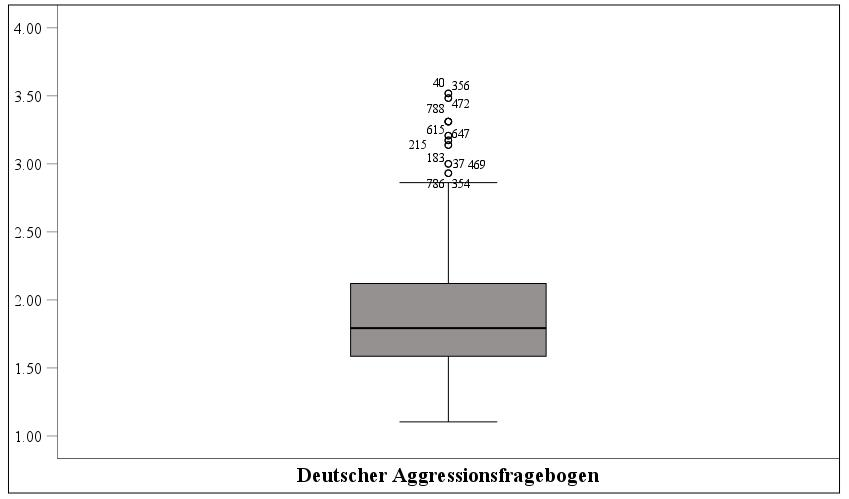
\includegraphics[width=\textwidth]{Boxplot AggroFB.jpg}
            %\caption[Linearer Zusammenhang des Deutschen Aggressionsfragebogens und des DVMAS]{Linearer Zusammenhang des Deutschen Aggressionsfragebogens und des DVMAS}

    \end{figure}
    
    

    %%%%%%%%%%%%%%%%%%%%%%%%%%%%%%%%%%%%%%%%%%%%

    \chapter{Boxplot DVMAS}            \label{Boxplot_DVMAS}
    %\addcontentsline{toc}{chapter}{B}
    \noindent \textit{Boxplot zur Erfassung der Ausreißer des DVMAS}

    \begin{figure}[htb!]
        \centering
            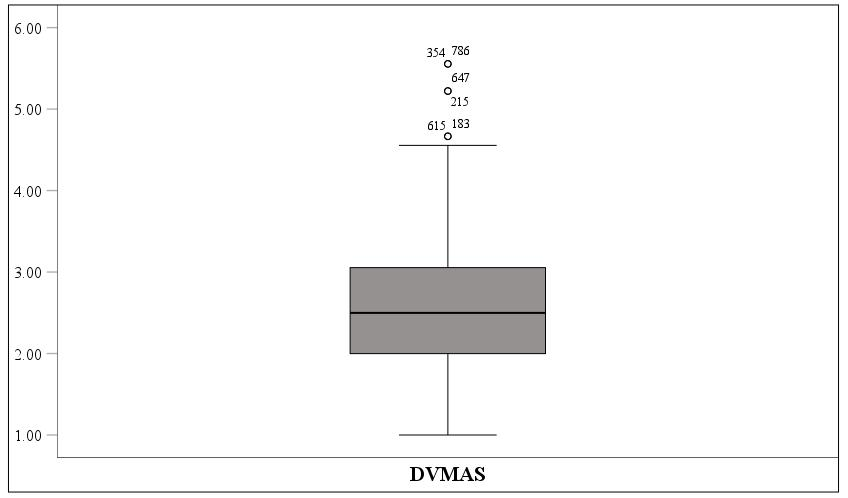
\includegraphics[width=\textwidth]{Boxplot DVMAS.jpg}
            %\caption[Linearer Zusammenhang des Deutschen Aggressionsfragebogens und des DVMAS]{Linearer Zusammenhang des Deutschen Aggressionsfragebogens und des DVMAS}

    \end{figure}
    
    

%%%%%%%%%%%%%%%%%%%%%%%%%%%%%%%%%%%%%%%%%%%%

\chapter{Linearität Deutscher Aggressionsfragebogen und DVMAS} \label{Linearitat_AggroFB_DVMAS}
%\addcontentsline{toc}{chapter}{C}
\noindent \textit{Linearer Zusammenhang des Deutschen Aggressionsfragebogens und des DVMAS}

\begin{figure}[htb!]
    \centering
        \includegraphics[width=\textwidth]{Linearität AggroFB-DVMAS.jpg}
        %\caption[Linearer Zusammenhang des Deutschen Aggressionsfragebogens und des DVMAS]{Linearer Zusammenhang des Deutschen Aggressionsfragebogens und des DVMAS}
        
\end{figure}
    
    

%%%%%%%%%%%%%%%%%%%%%%%%%%%%%%%%%%%%%%%%%%%%

    \chapter{Boxplot Aggression$-$Subskala physische Aggression}            \label{Boxplot_phAggro}
    %\addcontentsline{toc}{chapter}{D}
    \noindent \textit{Boxplot zur Erfassung der Ausreißer der Aggression$-$Subskala physische Aggression}

    \begin{figure}[htb!]
        \centering
            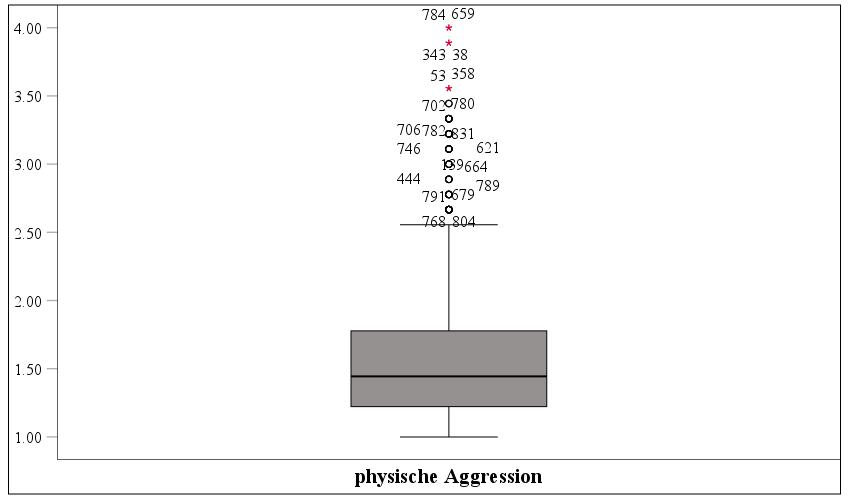
\includegraphics[width=\textwidth]{Boxplot ph_aggro.jpg}
            %\caption[Linearer Zusammenhang des Deutschen Aggressionsfragebogens und des DVMAS]{Linearer Zusammenhang des Deutschen Aggressionsfragebogens und des DVMAS}

    \end{figure}
    
    

%%%%%%%%%%%%%%%%%%%%%%%%%%%%%%%%%%%%%%%%%%%%

    \chapter{Online$-$Fragebogen}  \label{Fragebogen}
    %\addcontentsline{toc}{chapter}{E}
    \noindent \textit{Bildaufnahmen des Online$-$Fragbogens}

    \begin{figure}[htb!]
        \centering
            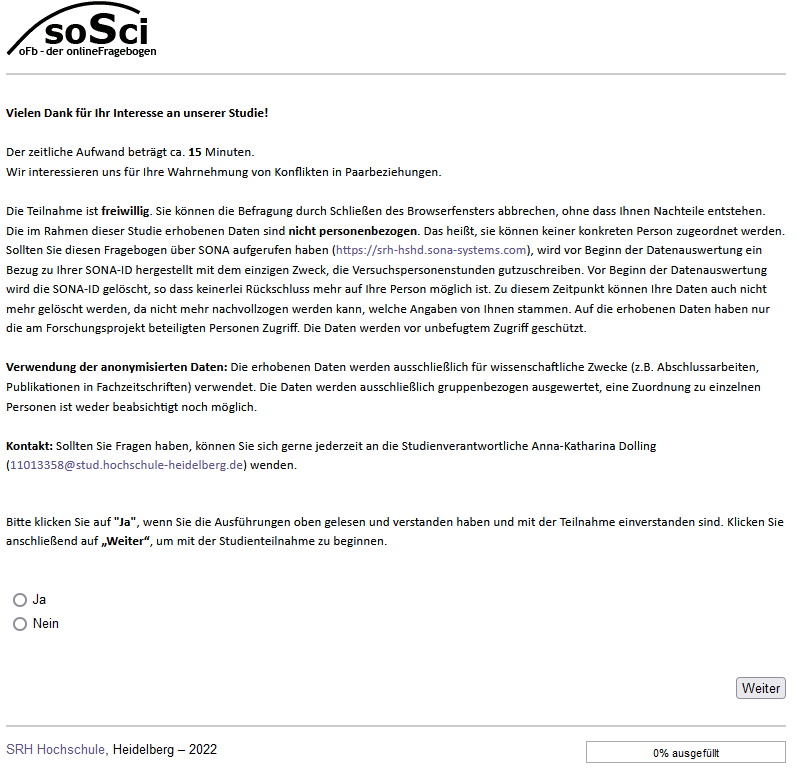
\includegraphics[width=\textwidth]{Seite 1.png}
            \caption[]{Seite 1 des Online$-$Fragebogens}
    \end{figure}

    \newpage
    \begin{figure}[htb!]
        \centering
            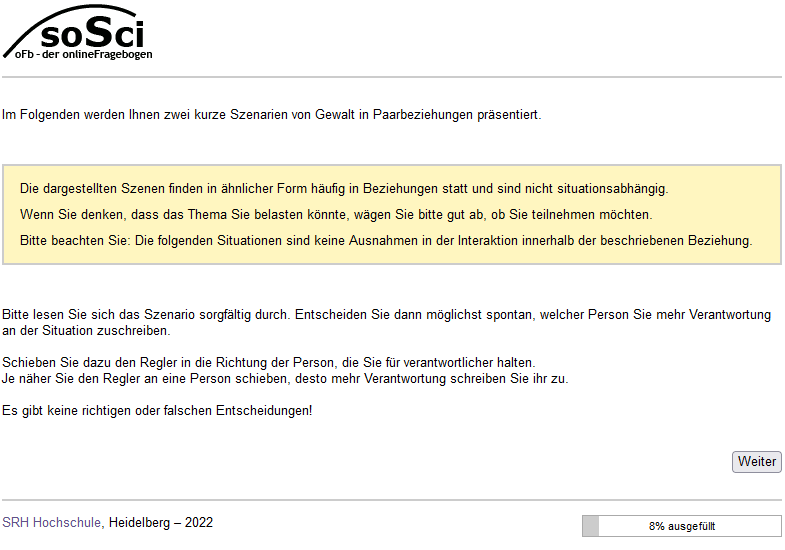
\includegraphics[width=\textwidth]{Seite 2.png}
            \caption[]{Seite 2 des Online$-$Fragebogens}
    \end{figure}

    \begin{figure}[htb!]
        \centering
            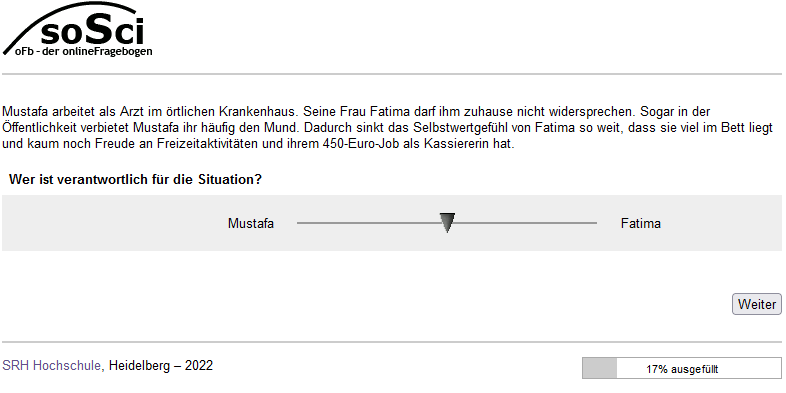
\includegraphics[width=\textwidth]{Seite 3.png}
            \caption[]{Seite 3 des Online$-$Fragebogens}
    \end{figure}
    
    \newpage
    \begin{figure}[htb!]
        \centering
            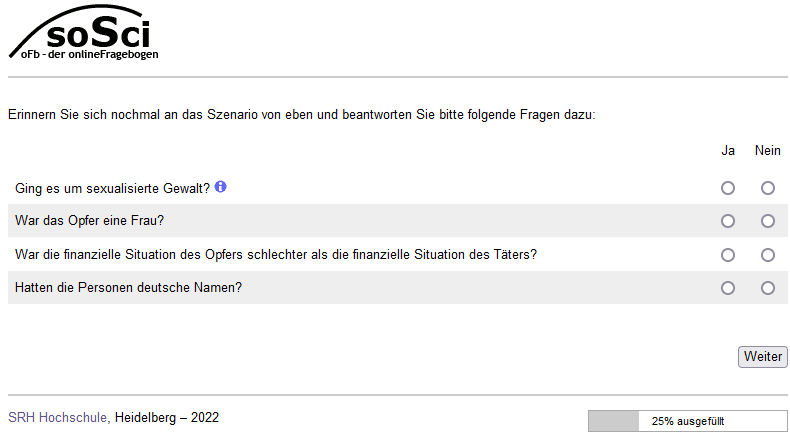
\includegraphics[width=\textwidth]{Seite 4.png}
            \caption[]{Seite 4 des Online$-$Fragebogens}
    \end{figure}
    
    \begin{figure}[htb!]
        \centering
            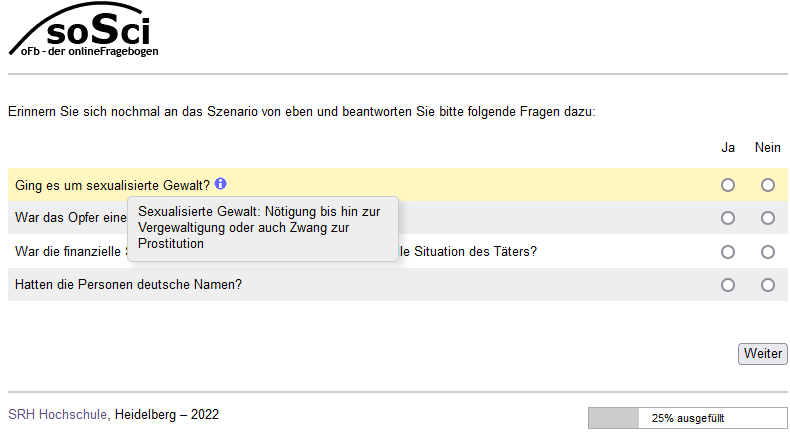
\includegraphics[width=\textwidth]{Seite 4 mit Infobox.png}
            \caption[]{Seite 4 des Online$-$Fragebogens mit Infobox}
    \end{figure}
    
    \newpage
    \begin{figure}[htb!]
        \centering
            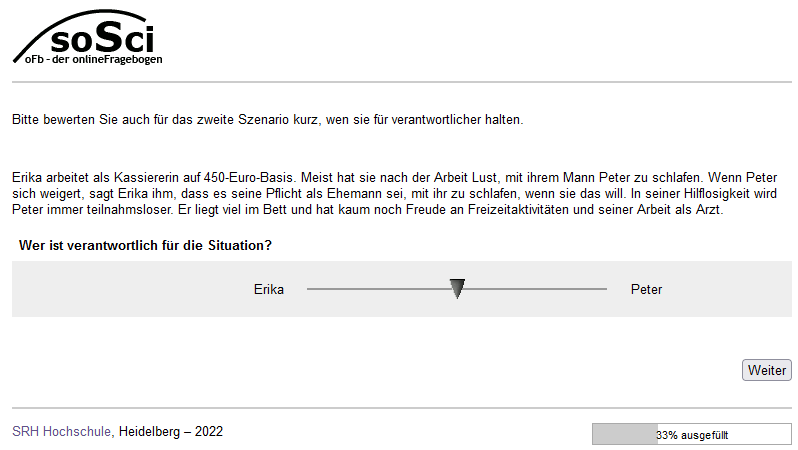
\includegraphics[width=\textwidth]{Seite 5.png}
            \caption[]{Seite 5 des Online$-$Fragebogens}
    \end{figure}
    
    \begin{figure}[htb!]
        \centering
            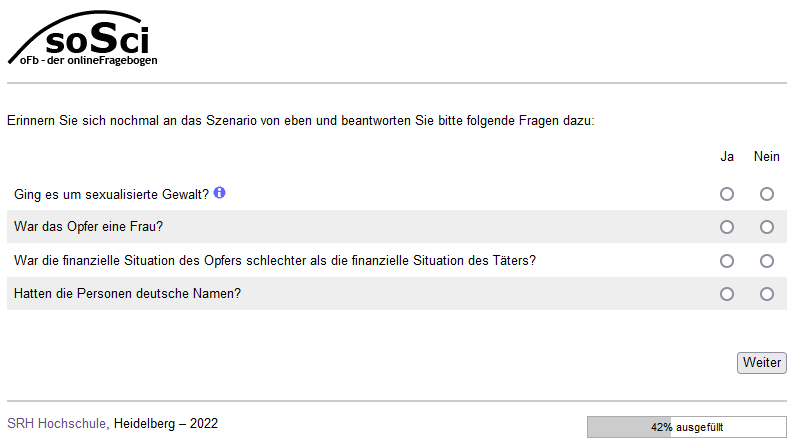
\includegraphics[width=\textwidth]{Seite 6.png}
            \caption[]{Seite 6 des Online$-$Fragebogens}
    \end{figure}
    
    \newpage
    \begin{figure}[htb!]
        \centering
            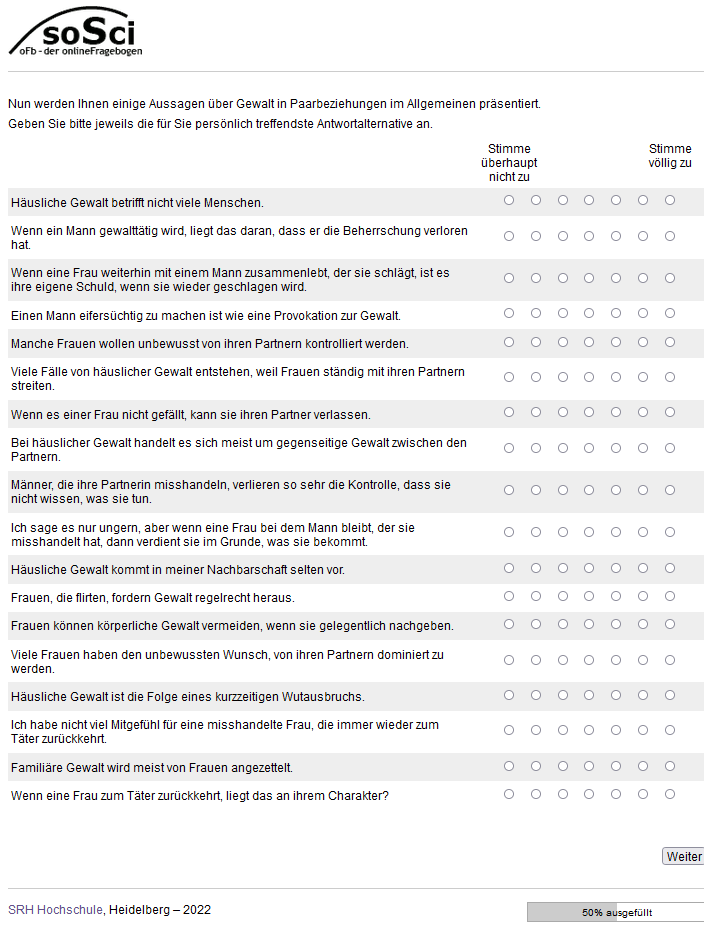
\includegraphics[width=\textwidth]{Seite 7.png}
            \caption[]{Seite 7 des Online$-$Fragebogens (deutsche Übersetzung des englischen DVMAS nach \textcite{Peters2003})}
    \end{figure}
    
    \newpage
    \begin{figure}[htb!]
        \centering
            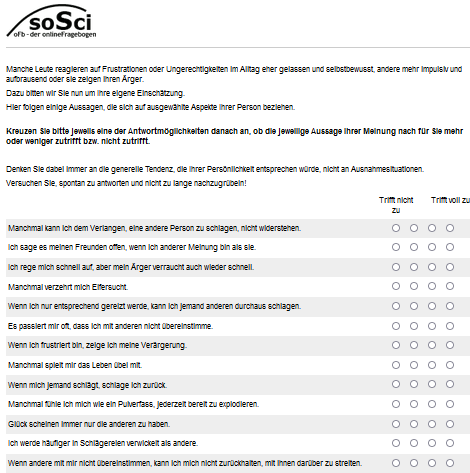
\includegraphics[width=\textwidth]{Seite 8_1.png}
            \caption[]{Erste Hälfte von Seite 8 des Online$-$Fragebogens des Deutschen Aggressionsfragebogens \parencite{Aggressionsfragebogen}}
    \end{figure}
    
    \newpage
    \begin{figure}[htb!]
        \centering
            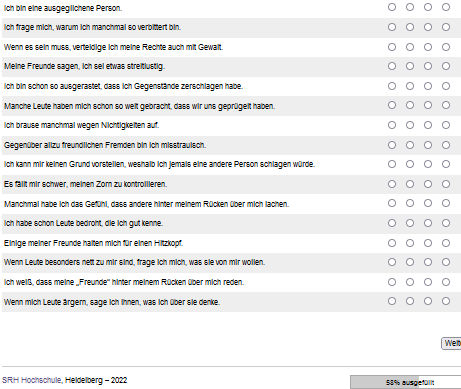
\includegraphics[width=\textwidth]{Seite 8_2.png}
            \caption[]{Zweite Hälfte von Seite 8 des Online$-$Fragebogens des Deutschen Aggressionsfragebogens \parencite{Aggressionsfragebogen}}
    \end{figure}
    
    \newpage
    \begin{figure}[htb!]
        \centering
            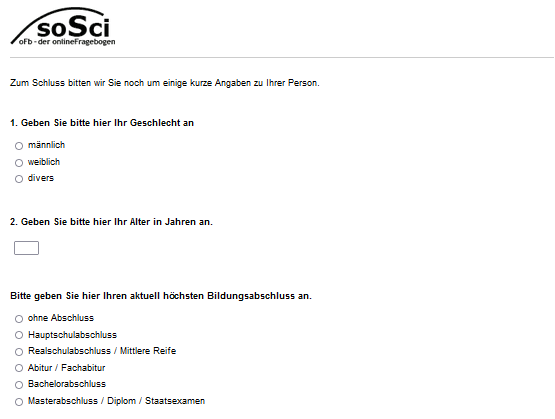
\includegraphics[width=\textwidth]{Seite 9_1.png}
            \caption[]{Erste Hälfte von Seite 9 des Online$-$Fragebogens}
    \end{figure}
    
    \newpage
    \begin{figure}[htb!]
        \centering
            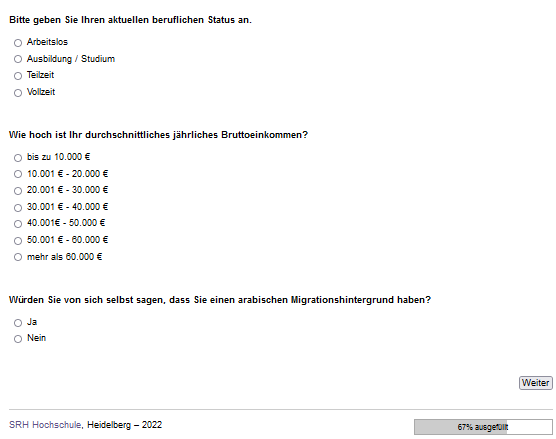
\includegraphics[width=\textwidth]{Seite 9_2.png}
            \caption[]{Zweite Hälfte von Seite 9 des Online$-$Fragebogens}
    \end{figure}
    
    \begin{figure}[htb!]
        \centering
            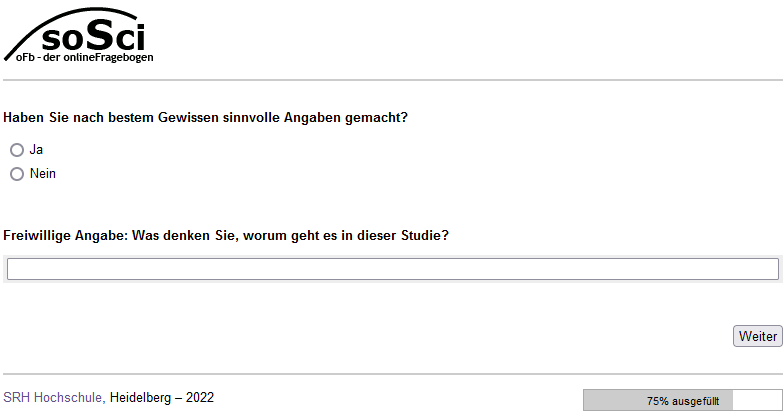
\includegraphics[width=\textwidth]{Seite 10.png}
            \caption[]{Seite 10 des Online$-$Fragebogens}
    \end{figure}
    
    \newpage
    \begin{figure}[htb!]
        \centering
            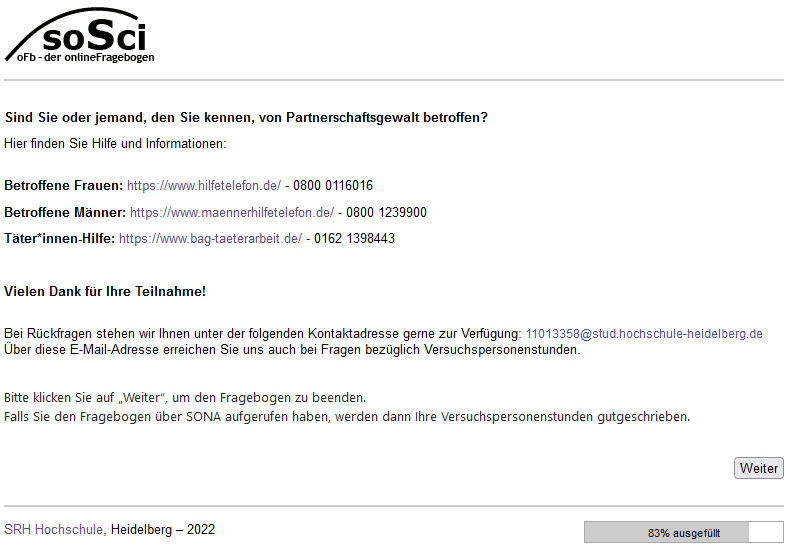
\includegraphics[width=\textwidth]{Seite 11.png}
            \caption[]{Seite 11 des Online$-$Fragebogens}
    \end{figure}
    
    \begin{figure}[htb!]
        \centering
            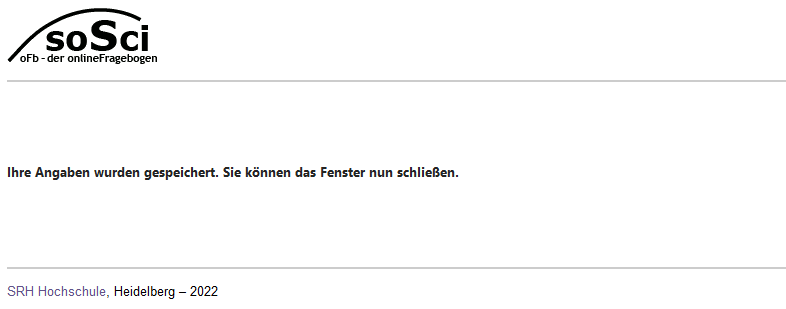
\includegraphics[width=\textwidth]{Seite 12.png}
            \caption[]{Seite 12 des Online$-$Fragebogens}
    \end{figure}


    
    

%%%%%%%%%%%%%%%%%%%%%%%%%%%%%%%%%%%%%%%%%%%%
\end{appendices}







%%%%%%%%% wenn mehrere Anhänge vorhanden %%%%%%%%%



%%%%%%%%% wenn nur 1 Anhang vorhanden %%%%%%%%%
%\chapter*{Anhang}
%\addcontentsline{toc}{chapter}{Anhang}
%\noindent \textit{Titel des Anhangs}

%Inhalt
%%%%%%%%% wenn nur 1 Anhang vorhanden %%%%%%%%%
%\clearpage
\newpage
\fontsize{18pt}{0pt}\textbf{Ehrenwörtliche Erklärung}
\parskip=32pt

\noindent Gemäß Studien- und Prüfungsordnung erklären wir, dass wir diese schriftliche 
Hausarbeit selbstständig angefertigt und wörtliche und sinngemäße Zitate 
kenntlich gemacht haben. Mit der Überprüfung auf etwaige Übereinstimmungen mit 
fremden Quellen mit Hilfe von Anti- Plagiatssoftware sind wir einverstanden. 
Wir erklären außerdem, dass diese Arbeit nicht im Rahmen eines anderen 
Prüfungsverfahrens bereits vorgelegt wurde. 
\parskip=32pt

\noindent Heidelberg, den \today
\parskip=32pt

\noindent Unterschriften:

[Unterschrift 1]

[Unterschrift 2]
\end{document}
